\documentclass[11pt,a4paper]{article}
\usepackage[a4paper,hmargin=1in,vmargin=1in]{geometry}
\usepackage{pgfplots}
\pgfplotsset{compat=1.17}

\usepackage[british]{babel}
\usepackage[utf8]{inputenc}
\usepackage[T1]{fontenc}

\usepackage[nodayofweek]{datetime}
\newdate{date}{17}{1}{2024}

\usepackage{stddoc}
\usepackage{subcaption}
\usepackage{makecell}


\begin{document}

    \pagenumbering{arabic}

    % Header
    \begin{center}
        {\LARGE\textbf{B2M17NKA - Project II}}\\[3mm]
        \begin{minipage}{0.4\textwidth}
            \begin{flushleft}
                \textsc{\displaydate{date}}
            \end{flushleft}
        \end{minipage}
        ~
        \begin{minipage}{0.4\textwidth}
            \begin{flushright}
                \textsc{Martin Šimák}
            \end{flushright}
        \end{minipage}
        \noindent\rule{14.5cm}{0.4pt}
    \end{center}

    \paragraph{Task} \emph{Design of a multi-band mobile phone antenna}
    \begin{enumerate}[label=\arabic*.]
        \item Design the following two antennas and create their models in an electromagnetic simulator.
        \begin{enumerate}[label=\Alph*.]
            \item \emph{Planar F-Inverted Antenna (PIFA)} for two (optionally three) bands: E-GSM ($880$ to $935\,\mathrm{MHz}$), DCS ($1710$ to $1880\,\mathrm{MHz}$), optionally UMTS ($1920$ to $2170\,\mathrm{MHz}$). The antenna should achieve the resonation of $|\Gamma(f)| < -12\,\mathrm{dB}$ on the resonating bands centre frequencies.
            \item \emph{Electrically small, folded monopole with a capacitive load} of two different lengths: $\lambda_0/10$ and $\lambda_0/20$. Design the antenna to work on the resonant frequency assigned in Project I. The antenna should achieve the resonation of $|\Gamma(f)| < -15\,\mathrm{dB}$ on the resonant frequency $f_{\mathrm{res}} = 1.8\,\mathrm{GHz}$.
        \end{enumerate}

        \item Fabricate antenna A with the help of the department. Assume a realistic size of the ground plate corresponding to the dimensions of a mobile phone. The ground plate will be the dielectric substrate Isola IS400 of dimensions $60 \times 120 \times 1\, \mathrm{mm}$, with one-sided copper cladding. The shorting pin will be present in the form of an iron, $10\, \mathrm{mm}$ high distance pillar -- a hexagonal prism with $5\, \mathrm{mm}$ distance between opposing edges. The antenna will be fed be an SMA connector (dimensions in the attached drawing) stripped of the Teflon (PTFE) dielectric beyond the flange. The conductive pattern will be cut out of a thin (thickness $35\, \mathrm{\mu m}$) copper foil using a plotter. This adhesive foil will be contacted onto a thin (thickness $0.5\, \mathrm{mm}$) PET-G dielectric plate which will be placed on top of the iron distance pillar serving as a short.
        
        During the design, special attention should be paid to the practical feasibility of fabrication, namely the dimensions of the SMA connector and the shorting pin, making a hole for the SMA-feed centre pin etc. Determine the required minimum distance of the centre of the shorting pin from the centre pin of the connector.
        \begin{table}[!ht]
            \centering
            \begin{tabular}{|c|c|c|c|}
                \hline
                Antenna component & Substrate & $\epsilon_r\,[-]$ & $\tan(\delta)\,[-]$\\
                \hline\hline
                Ground plate & Isola IS400 & $3.9$ & $0.02$\\
                \hline
                Pattern-carrying plate & PET-G & $2.4$ & $0.02$\\
                \hline
                Plastic distance pillars & Polyamide & $4$ & $0.05$\\
                \hline
            \end{tabular}
            \caption{\label{table:pifa-construction-parameters}Construction parameters of the PIFA components}
        \end{table}

        \item Measure the reflection from the fabricated antenna in the operating frequency bands.
        
        \item Plot the important antenna parameters of all designed antennas:
        \begin{enumerate}[label=4.\arabic*]
            \item reflection coefficient (simulated, include measured for antenna A),
            \item input impedance (simulated, include measured for antenna A),
            \item 3D radiation patterns and cuts in the $E$- and $H$-plane (simulated, both bands for antenna A).
        \end{enumerate}

        \item Determine the fundamental limits in the design bands.
        \begin{enumerate}[label=5.\arabic*]
            \item Plot the Chu's limit $Q_{\mathrm{min}}(ka)$ using the relations from McLean, Thal and Gustafsson%
                \footnote{Determine $\gamma_1^{\mathrm{norm}}$ for the used geometry of the modelled radiators.}
            for $ka \in [0.1,1]$.
            \item Calculate the quality factors $Q_{3\mathrm{dB}}$ and $Q_Z$ (Yaghjian and Best, IEEE TAP, 2005) for all (simulated and measured) antennas from the input impedance $Z_{\mathrm{in}}(\omega)$ and add them to the plot mentioned above.
            \item Summarize the parameters $ka$, $Q_{3\mathrm{dB}}$, $Q_{3\mathrm{dB}}/Q_{\mathrm{min}}$, $Q_Z$, $Q_Z/Q_{\mathrm{min}}$, $\mathit{BW}_{3\, \mathrm{dB}}$ and $\mathit{BW}_{Q_Z}$ of the designed radiators in a table and discuss the effectiveness of their miniaturization. Assume $100\, \%$ antenna efficiency and $Q_{\mathrm{min}} = Q_{\mathrm{Gustafsson}}$. Discuss the applicability and suitability of the individual limits.
        \end{enumerate}
    \end{enumerate}

\newpage
    \section{Antenna models}
        All the antennas were designed in CST Studio Suite in accordance with the respective assignments. The final models are shown in Figure~\ref{fig:antenna-models}.
        \begin{figure}[!ht]
            \centering
            \begin{subfigure}{.8\textwidth}
                \centering
                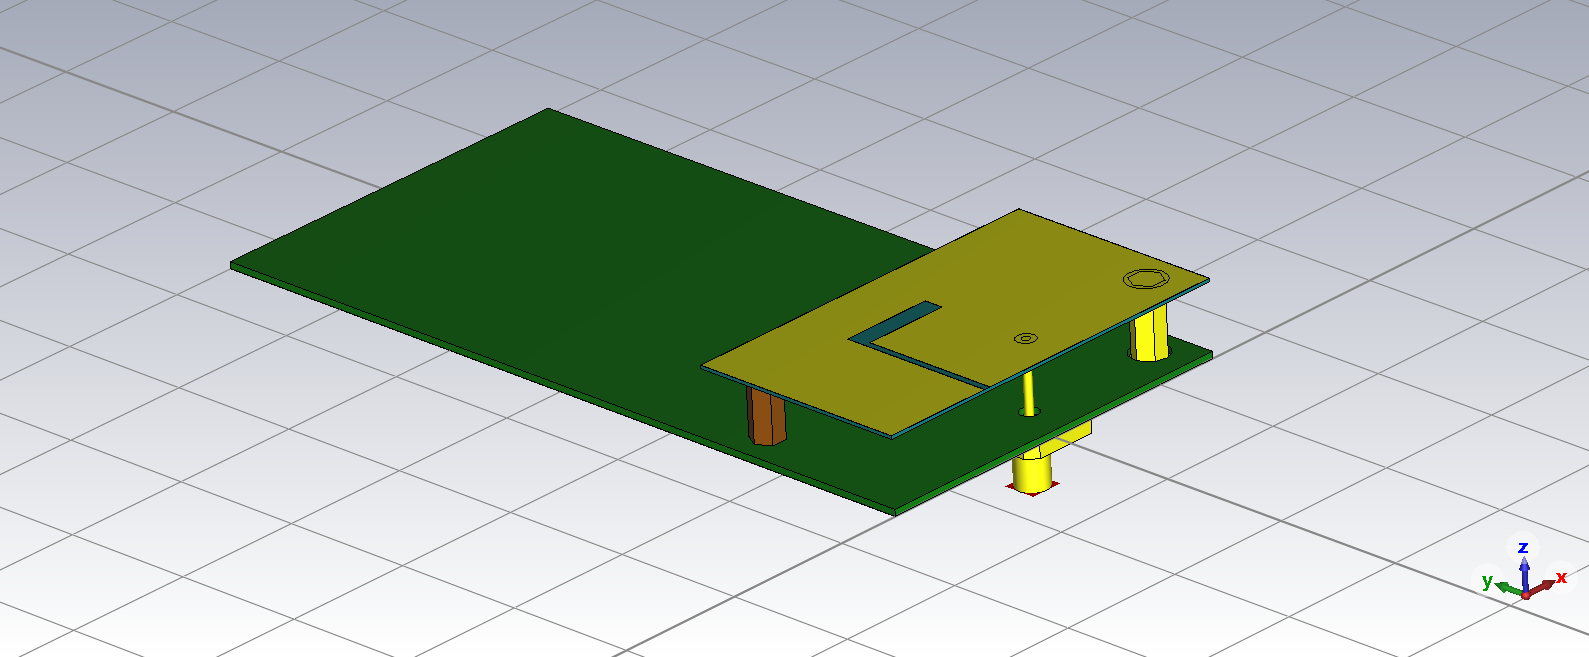
\includegraphics[width=\textwidth]{src/pifa-model.png}
                \caption{\label{fig:pifa-model}PIFA}
            \end{subfigure}
            \\[.5cm]
            \begin{subfigure}{.8\textwidth}
                \centering
                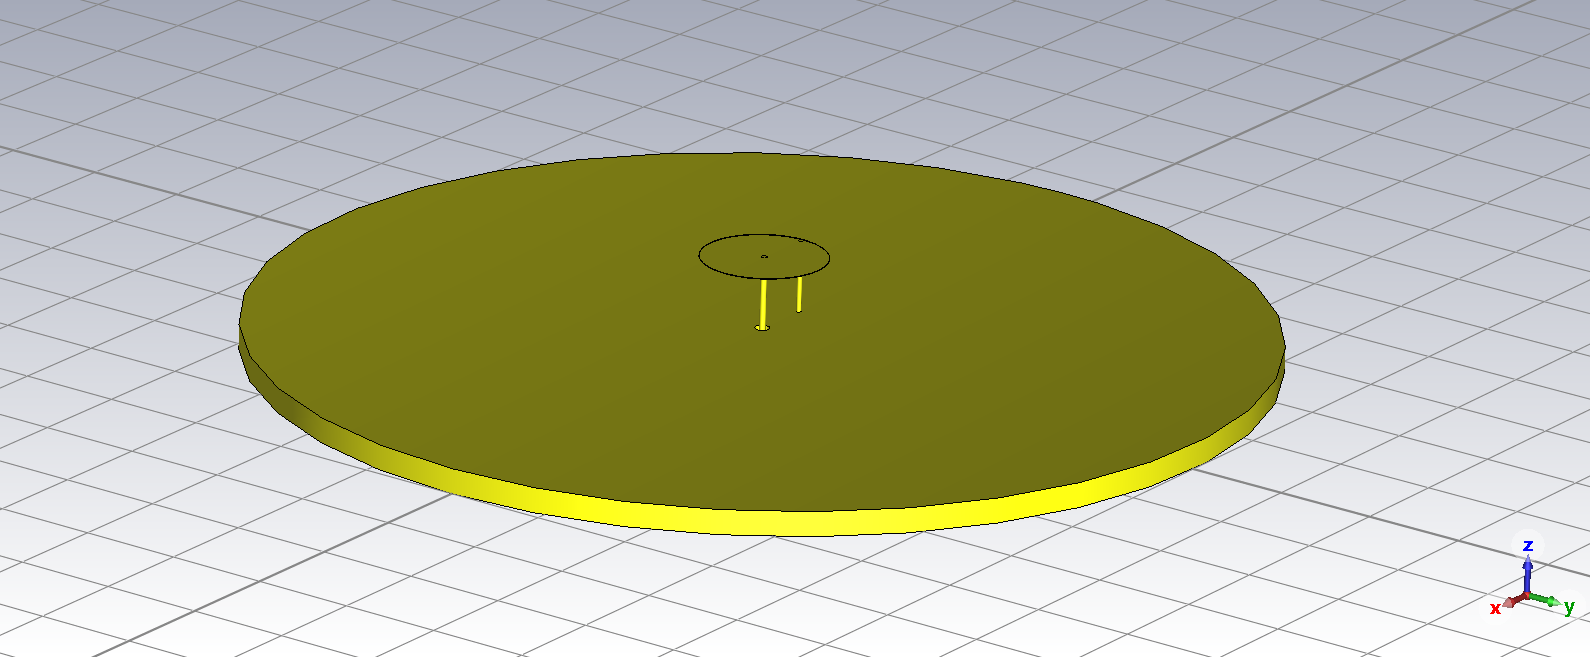
\includegraphics[width=\textwidth]{src/lambda-tenth-model.png}
                \caption{\label{fig:lambda-tenth-model}$\lambda/10$ monopole}
            \end{subfigure}
            \\[.5cm]
            \begin{subfigure}{.8\textwidth}
                \centering
                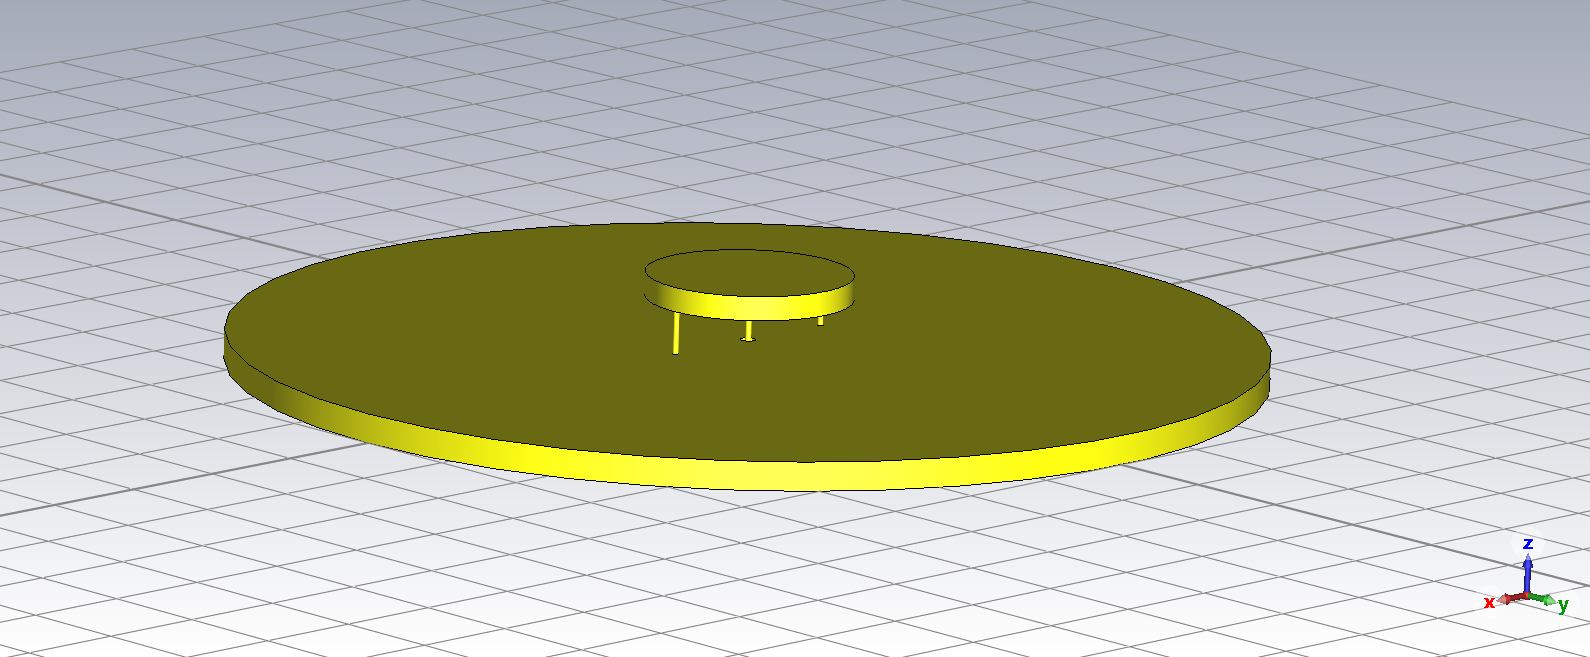
\includegraphics[width=\textwidth]{src/lambda-twentieth-model.png}
                \caption{\label{fig:lambda-twentieth-model}$\lambda/20$ monopole}
            \end{subfigure}
            \caption{\label{fig:antenna-models}Antenna models}
        \end{figure}

\newpage
    \section{PIFA fabrication}
        Antenna A (PIFA) has been successfully fabricated in one of the laboratory seminars during the semester. The final product is shown in Figure~\ref{fig:pifa-fabrication}. The distance of the centre of the shorting pin from the centre pin of the connector is $22.8\, \mathrm{mm}$.
        \begin{figure}[!ht]
            \centering
            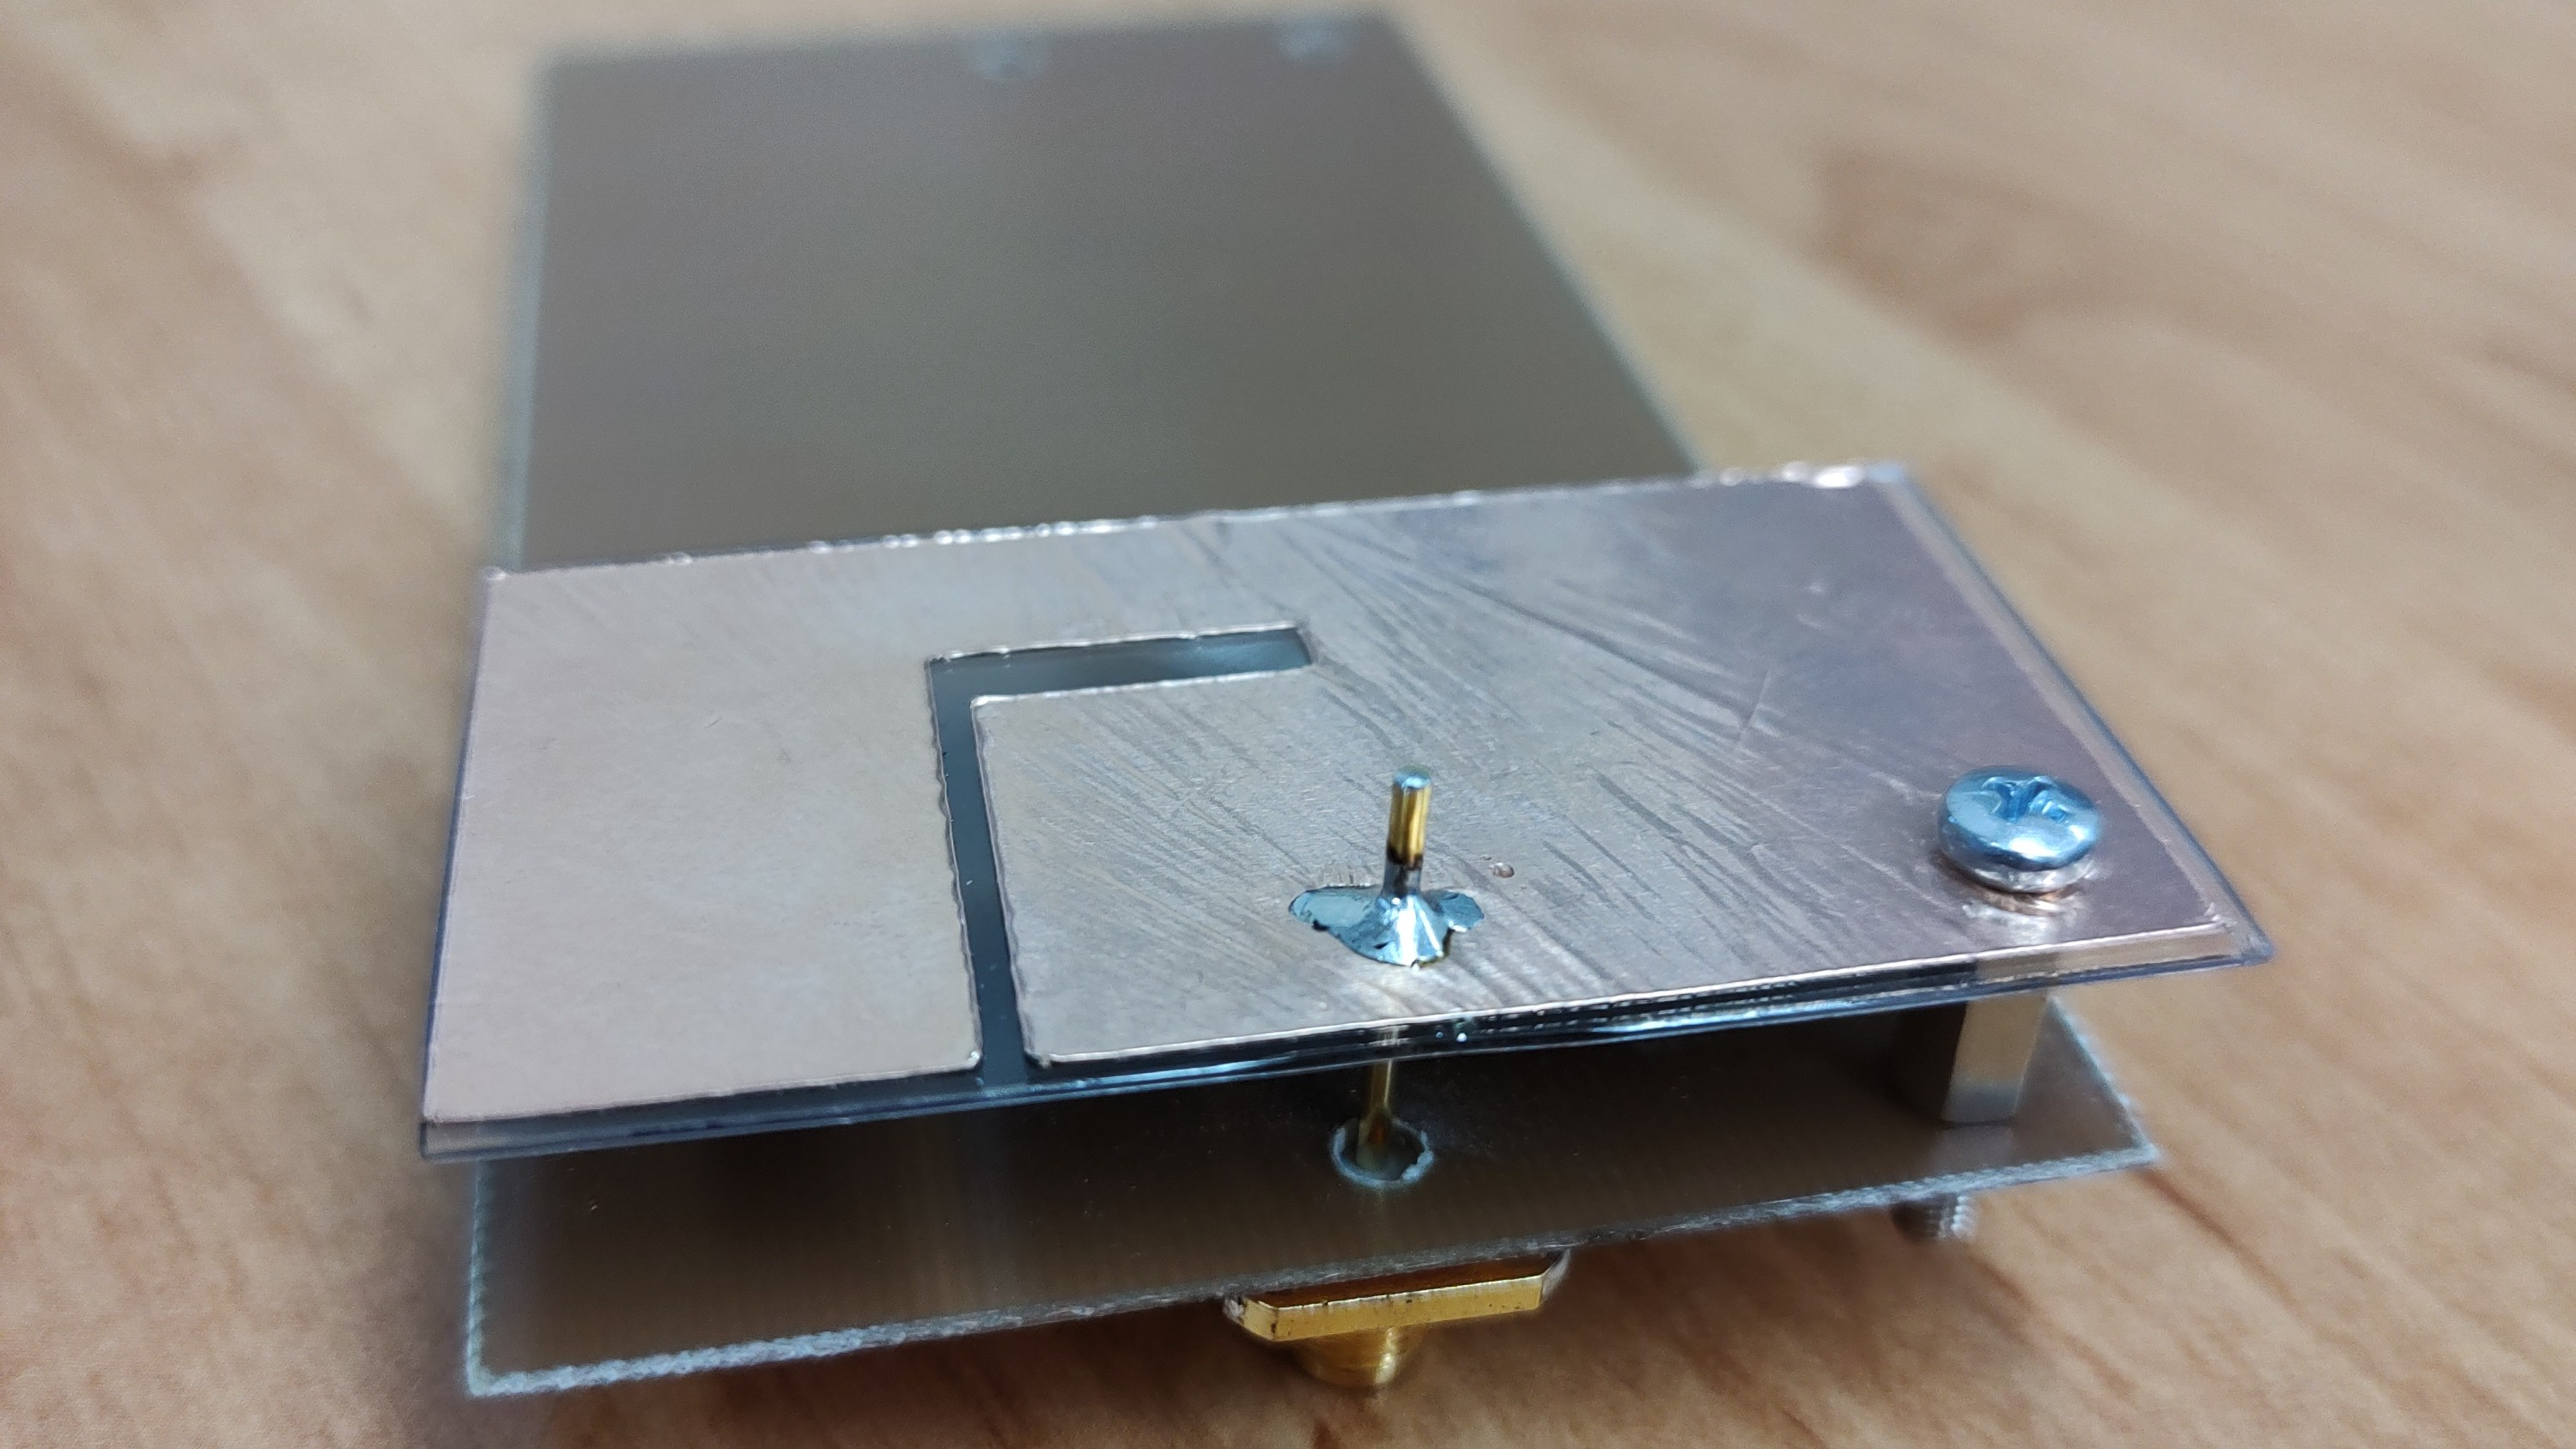
\includegraphics[width=.8\textwidth]{src/pifa-fabrication.jpg}
            \caption{\label{fig:pifa-fabrication}PIFA: fabrication}
        \end{figure}

    \section{Fabricated PIFA reflection measurement}
        The input impedance of the fabricated antenna A was determined from the S-parameters (reflection coefficient) measured using a VNA. The measured data is shown in Figure~\ref{fig:pifa-meas-reflection-linear}.
        \begin{figure}[!ht]
            \centering
            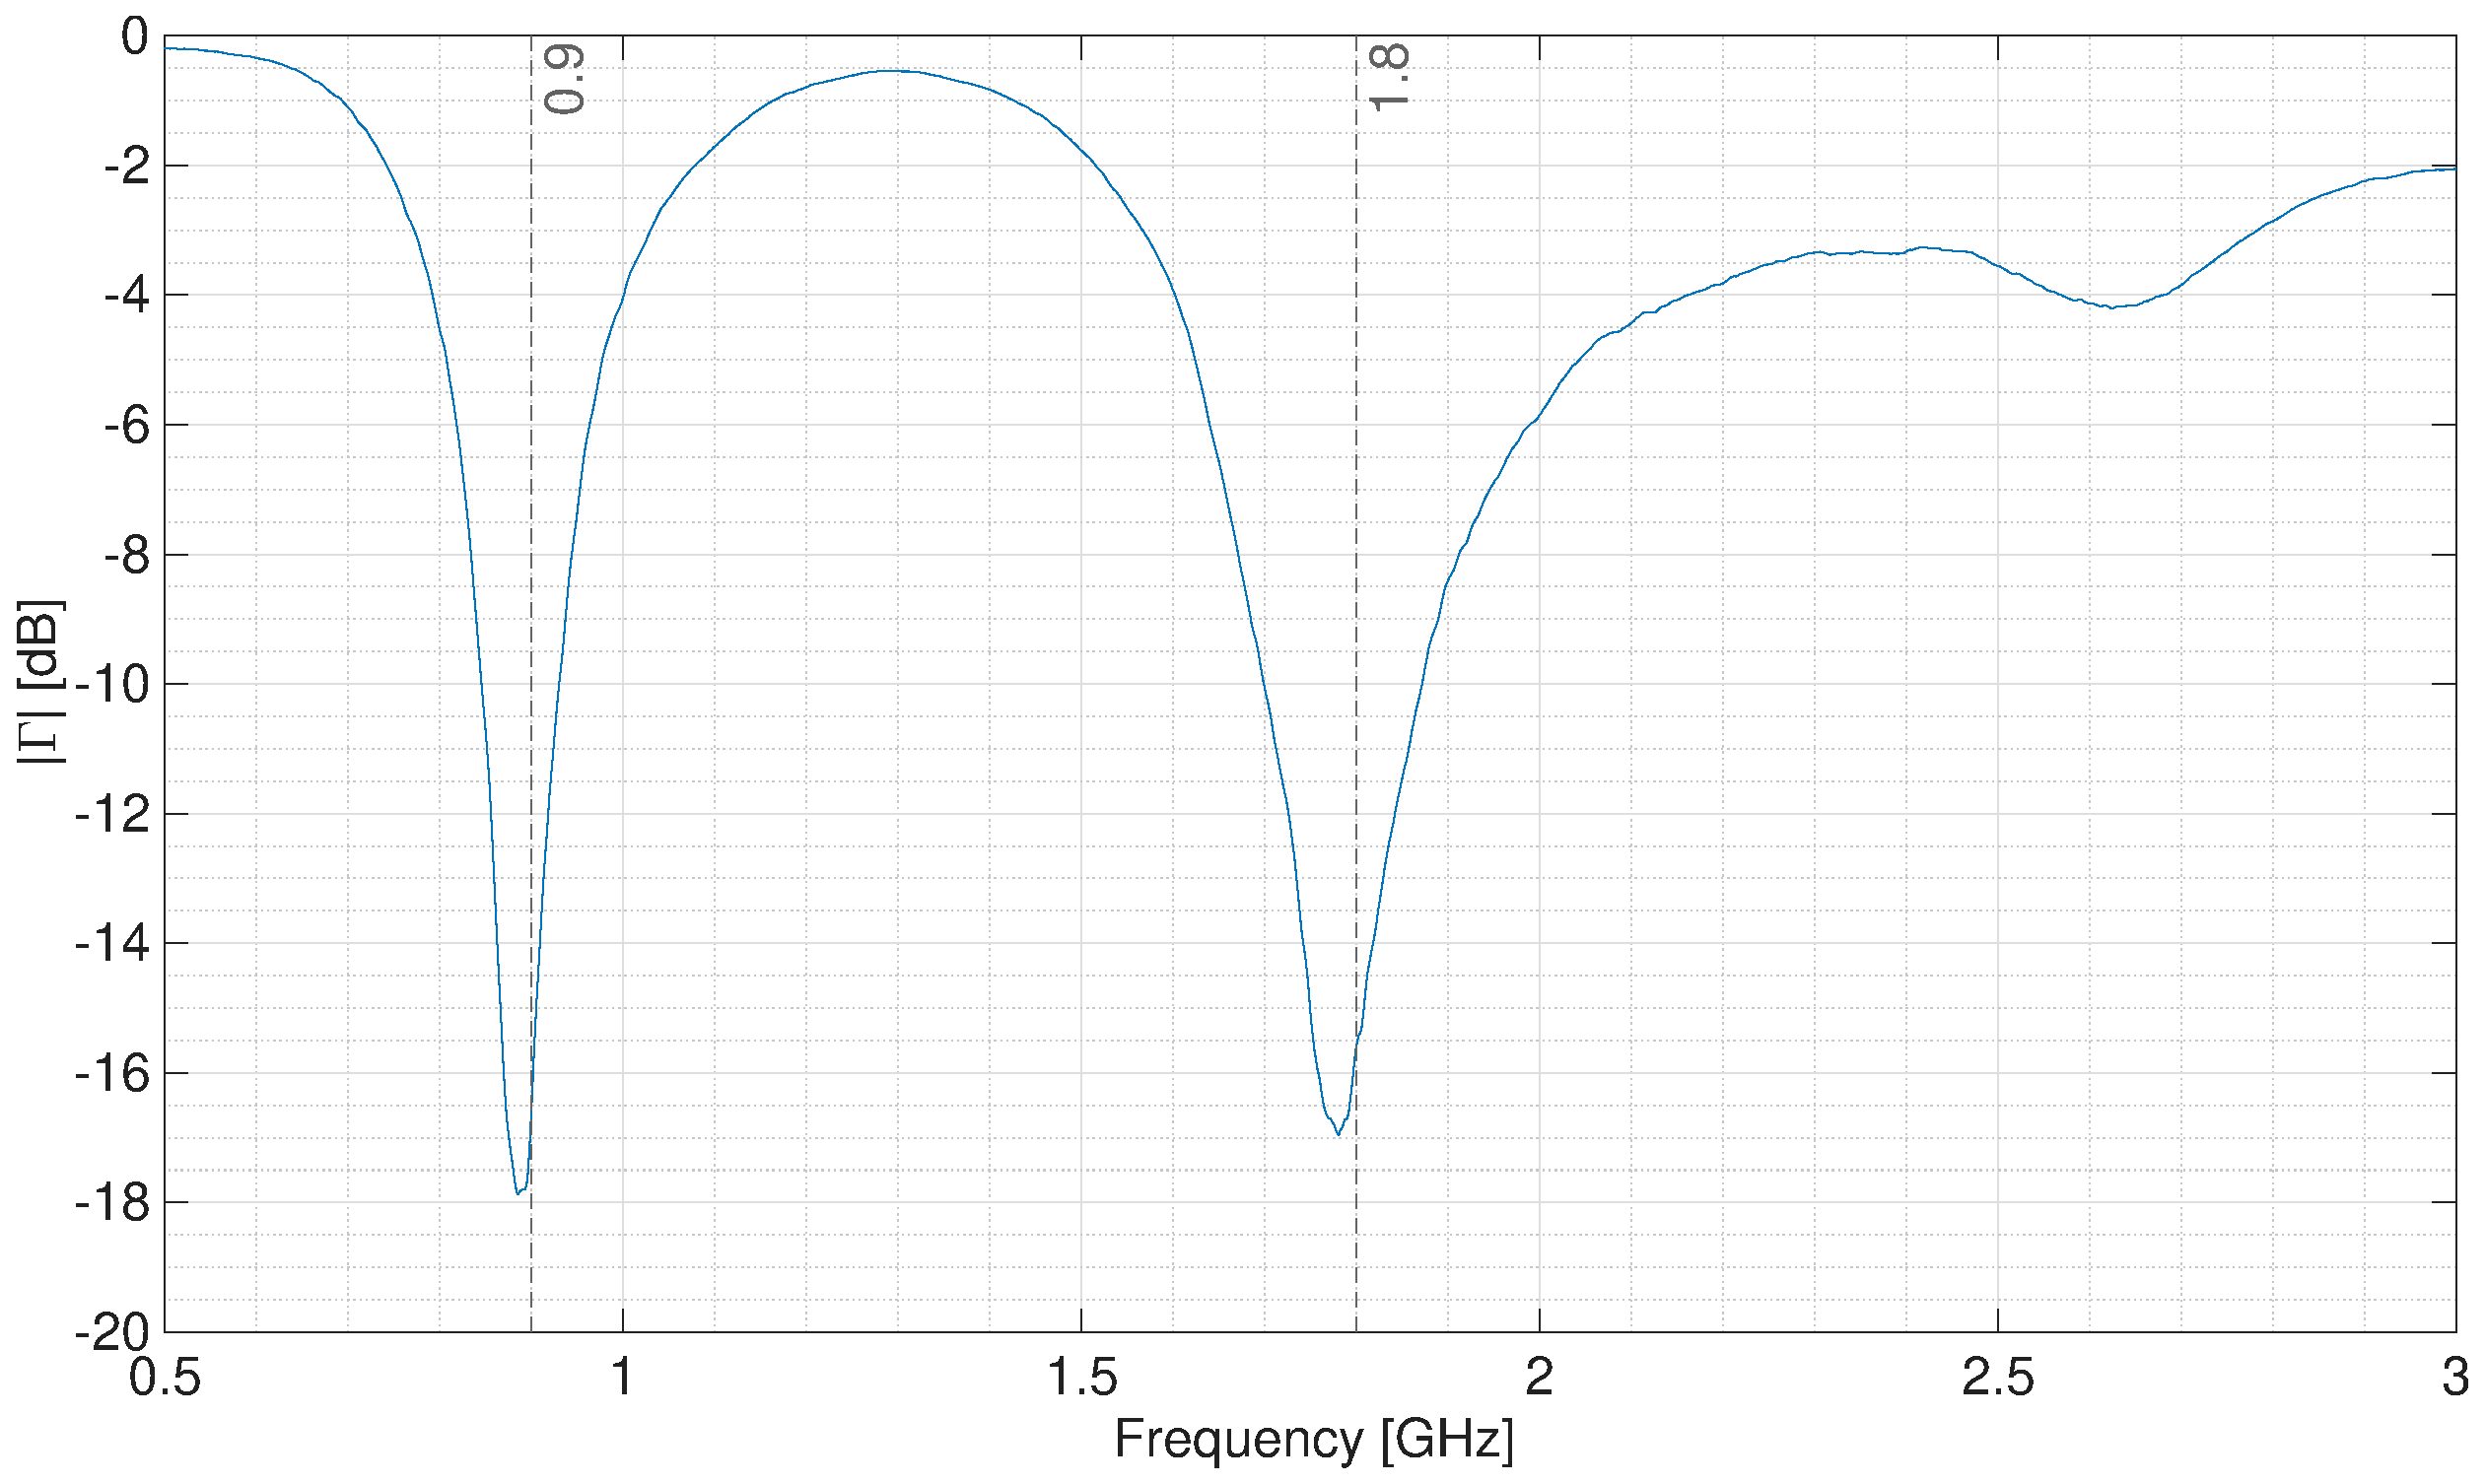
\includegraphics[width=.8\textwidth]{src/pifa-meas-reflection-linear.eps}
            \caption{\label{fig:pifa-meas-reflection-linear}PIFA: reflection measurement}
        \end{figure}

\newpage
    \section{Important antenna parameters}
        \paragraph{PIFA} The antenna was both designed and fabricated to the fulfilment of the assignment. This can be seen in Figure~\ref{fig:pifa-reflection-linear} where the magnitude of the reflection coefficient clearly reaches the expected values around both resonant frequencies. Furthermore, the complex reflection coefficient is shown using a Smith chart in Figure~\ref{fig:pifa-reflection-smith} and the input impedance is plotted by parts in Figure~\ref{fig:pifa-impedance}. The radiation properties are conveyed both in 3D and 2D. Figure~\ref{fig:pifa-farfield-0G9Hz} and Figure~\ref{fig:pifa-farfield-1G8Hz} show the 3D farfield pattern in the lower band and the upper band respectively. The radiation patterns can also be inspected in cuts through the $E$-plane in Figures~\ref{fig:pifa-radiation-e-0G9Hz}~and~\ref{fig:pifa-radiation-e-1G8Hz} for each band separately and through the $H$-plane in Figures~\ref{fig:pifa-radiation-h-0G9Hz}~and~\ref{fig:pifa-radiation-h-1G8Hz}.

        \begin{figure}[!ht]
            \centering
            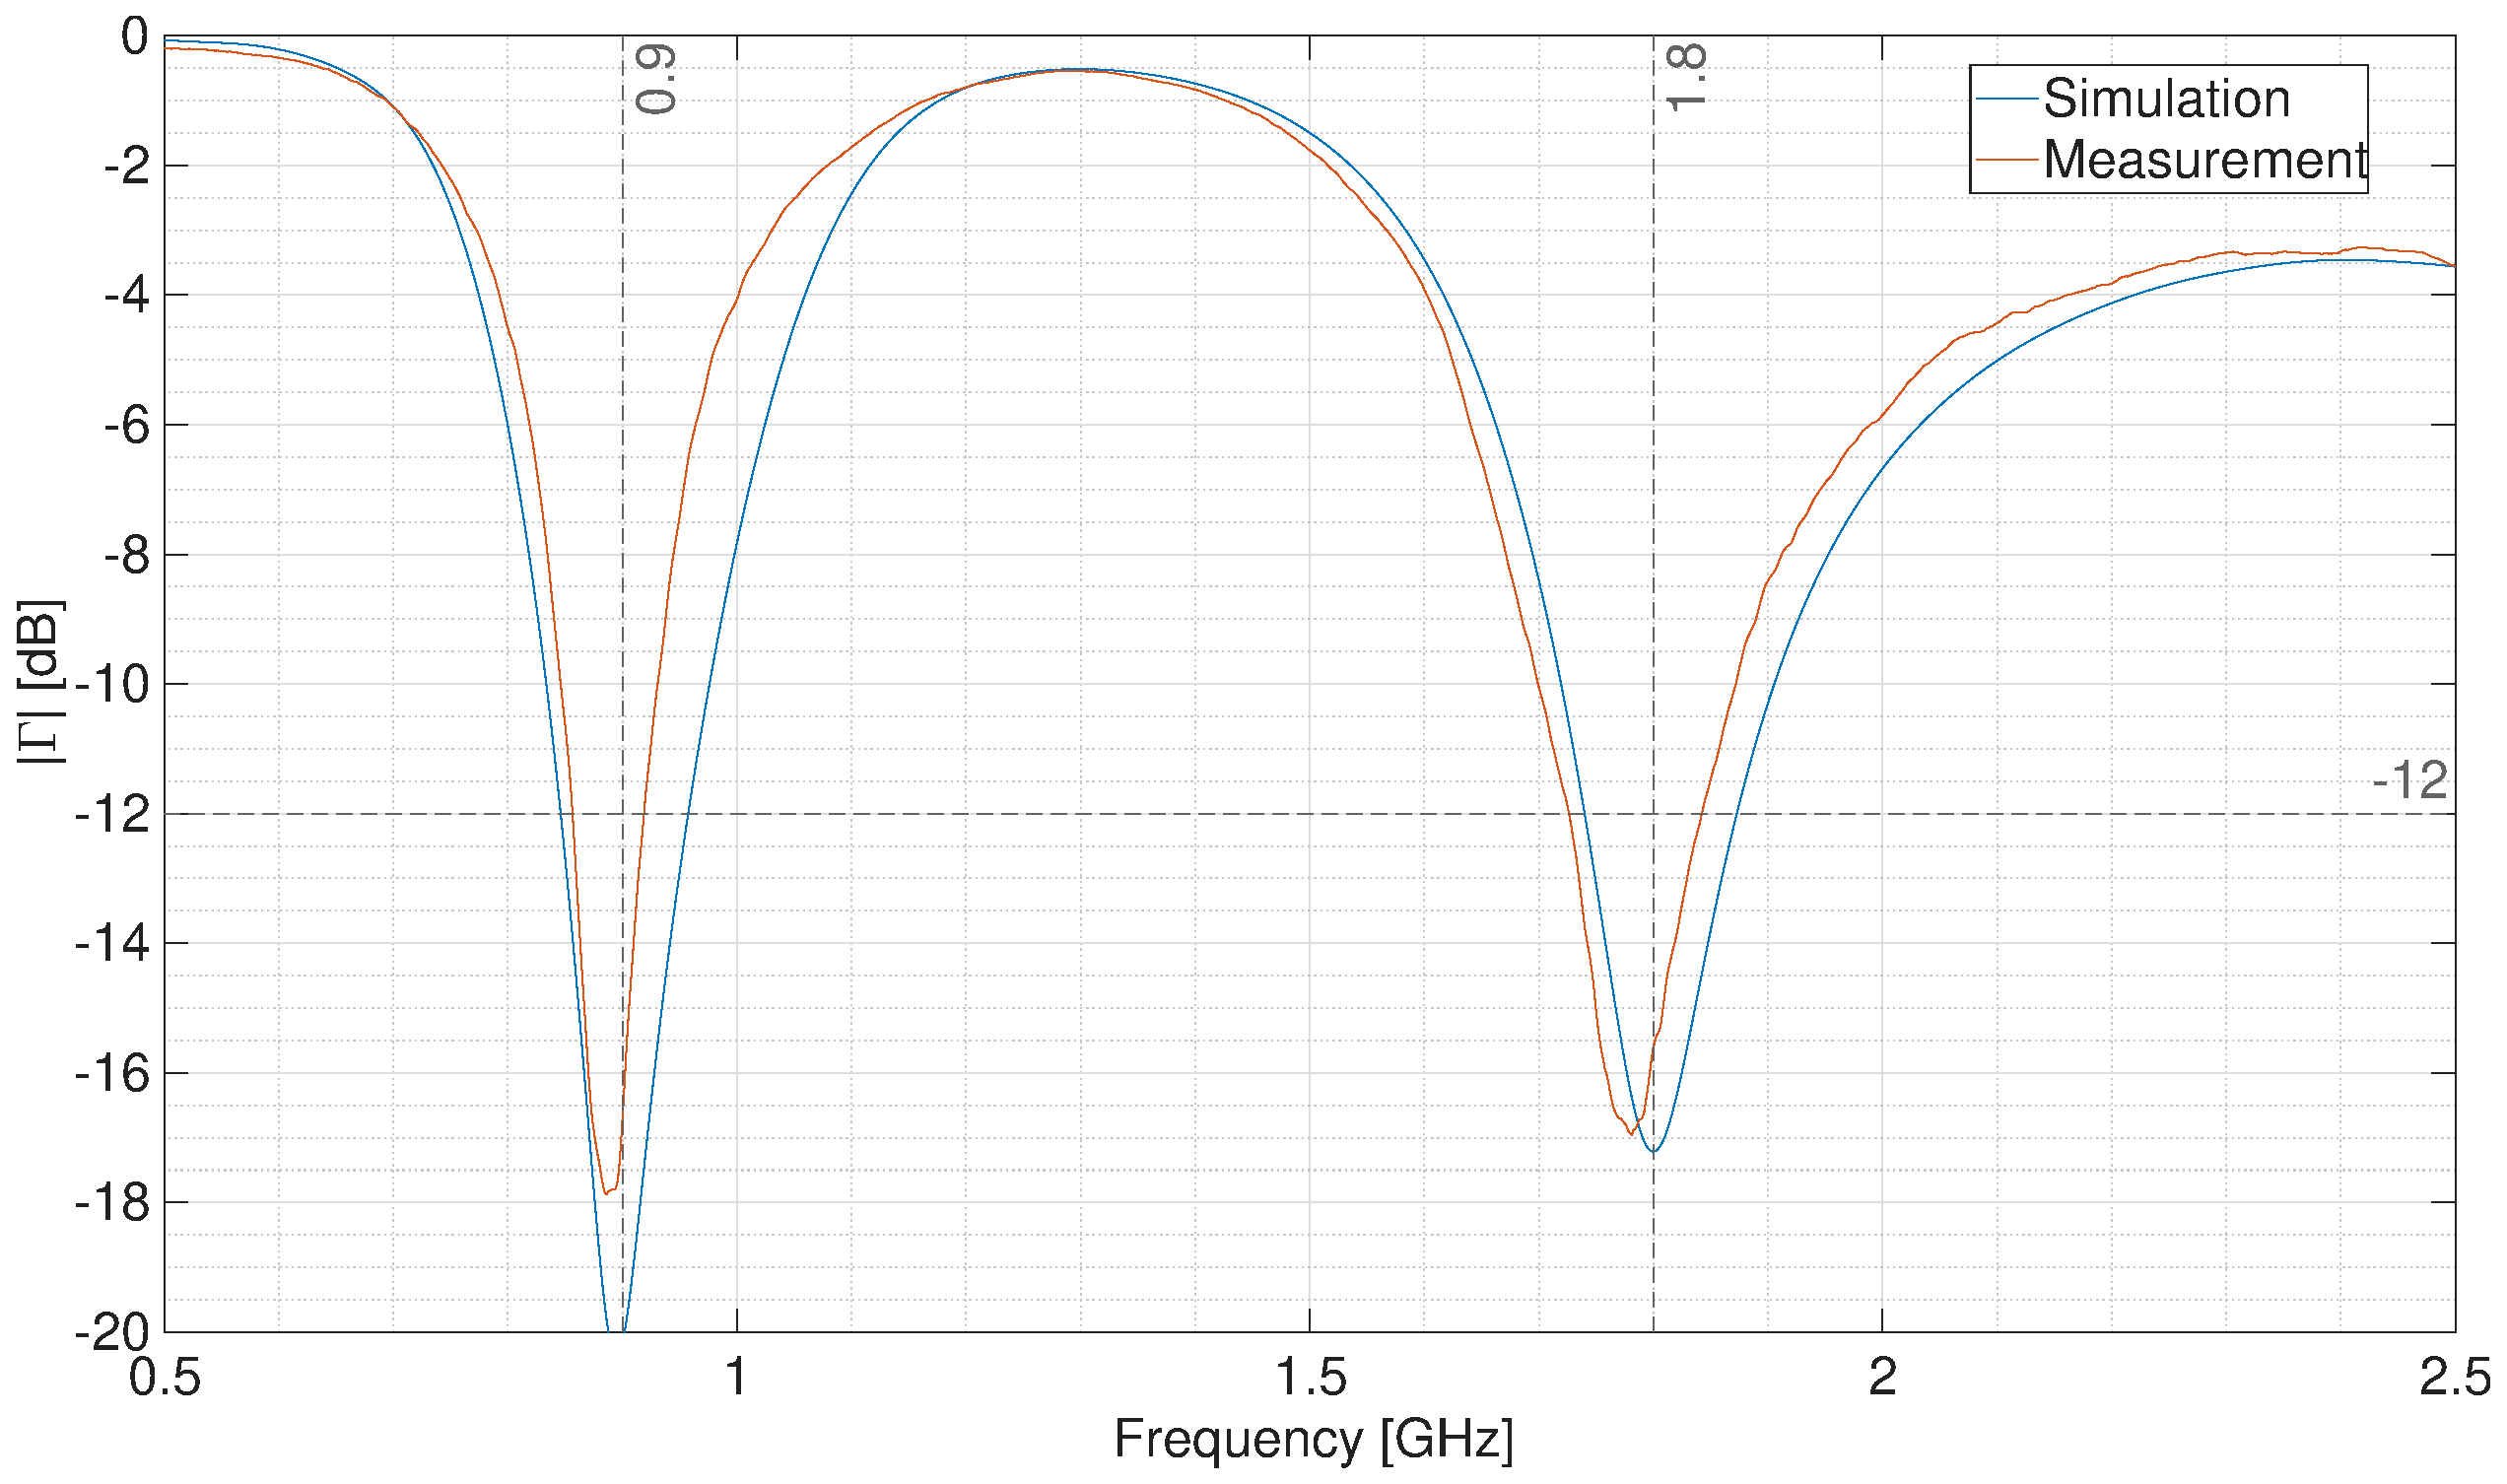
\includegraphics[width=.8\textwidth]{src/pifa-reflection-linear.eps}
            \caption{\label{fig:pifa-reflection-linear}PIFA: Reflection coefficient in the linear scale}
        \end{figure}
        
        \begin{figure}[!ht]
            \centering
            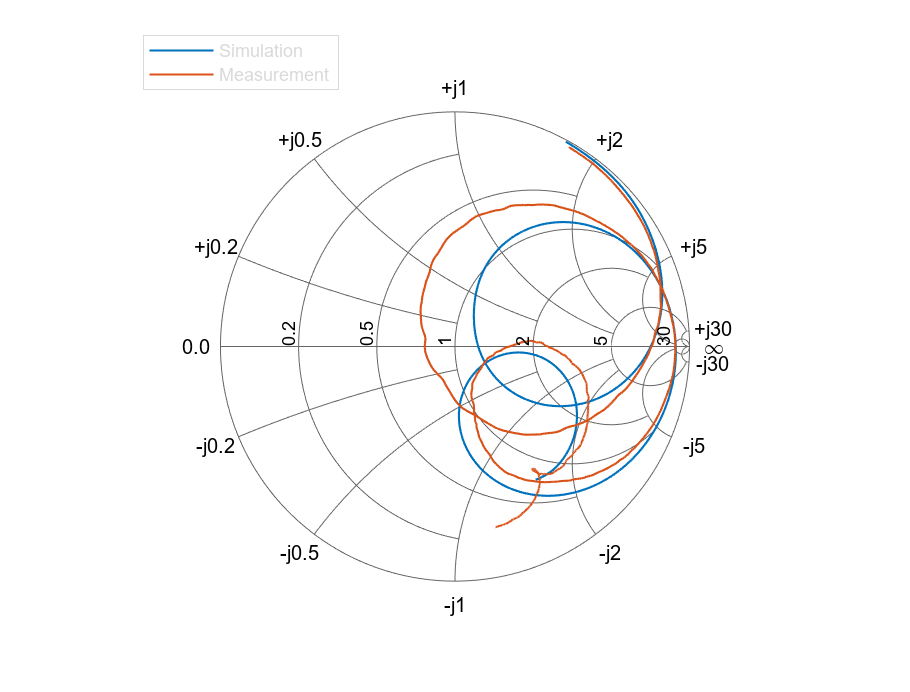
\includegraphics[width=.7\textwidth]{src/pifa-reflection-smith.eps}
            \caption{\label{fig:pifa-reflection-smith}PIFA: Reflection coefficient in the Smith chart}
        \end{figure}
        
\newpage
        \begin{figure}[!ht]
            \centering
            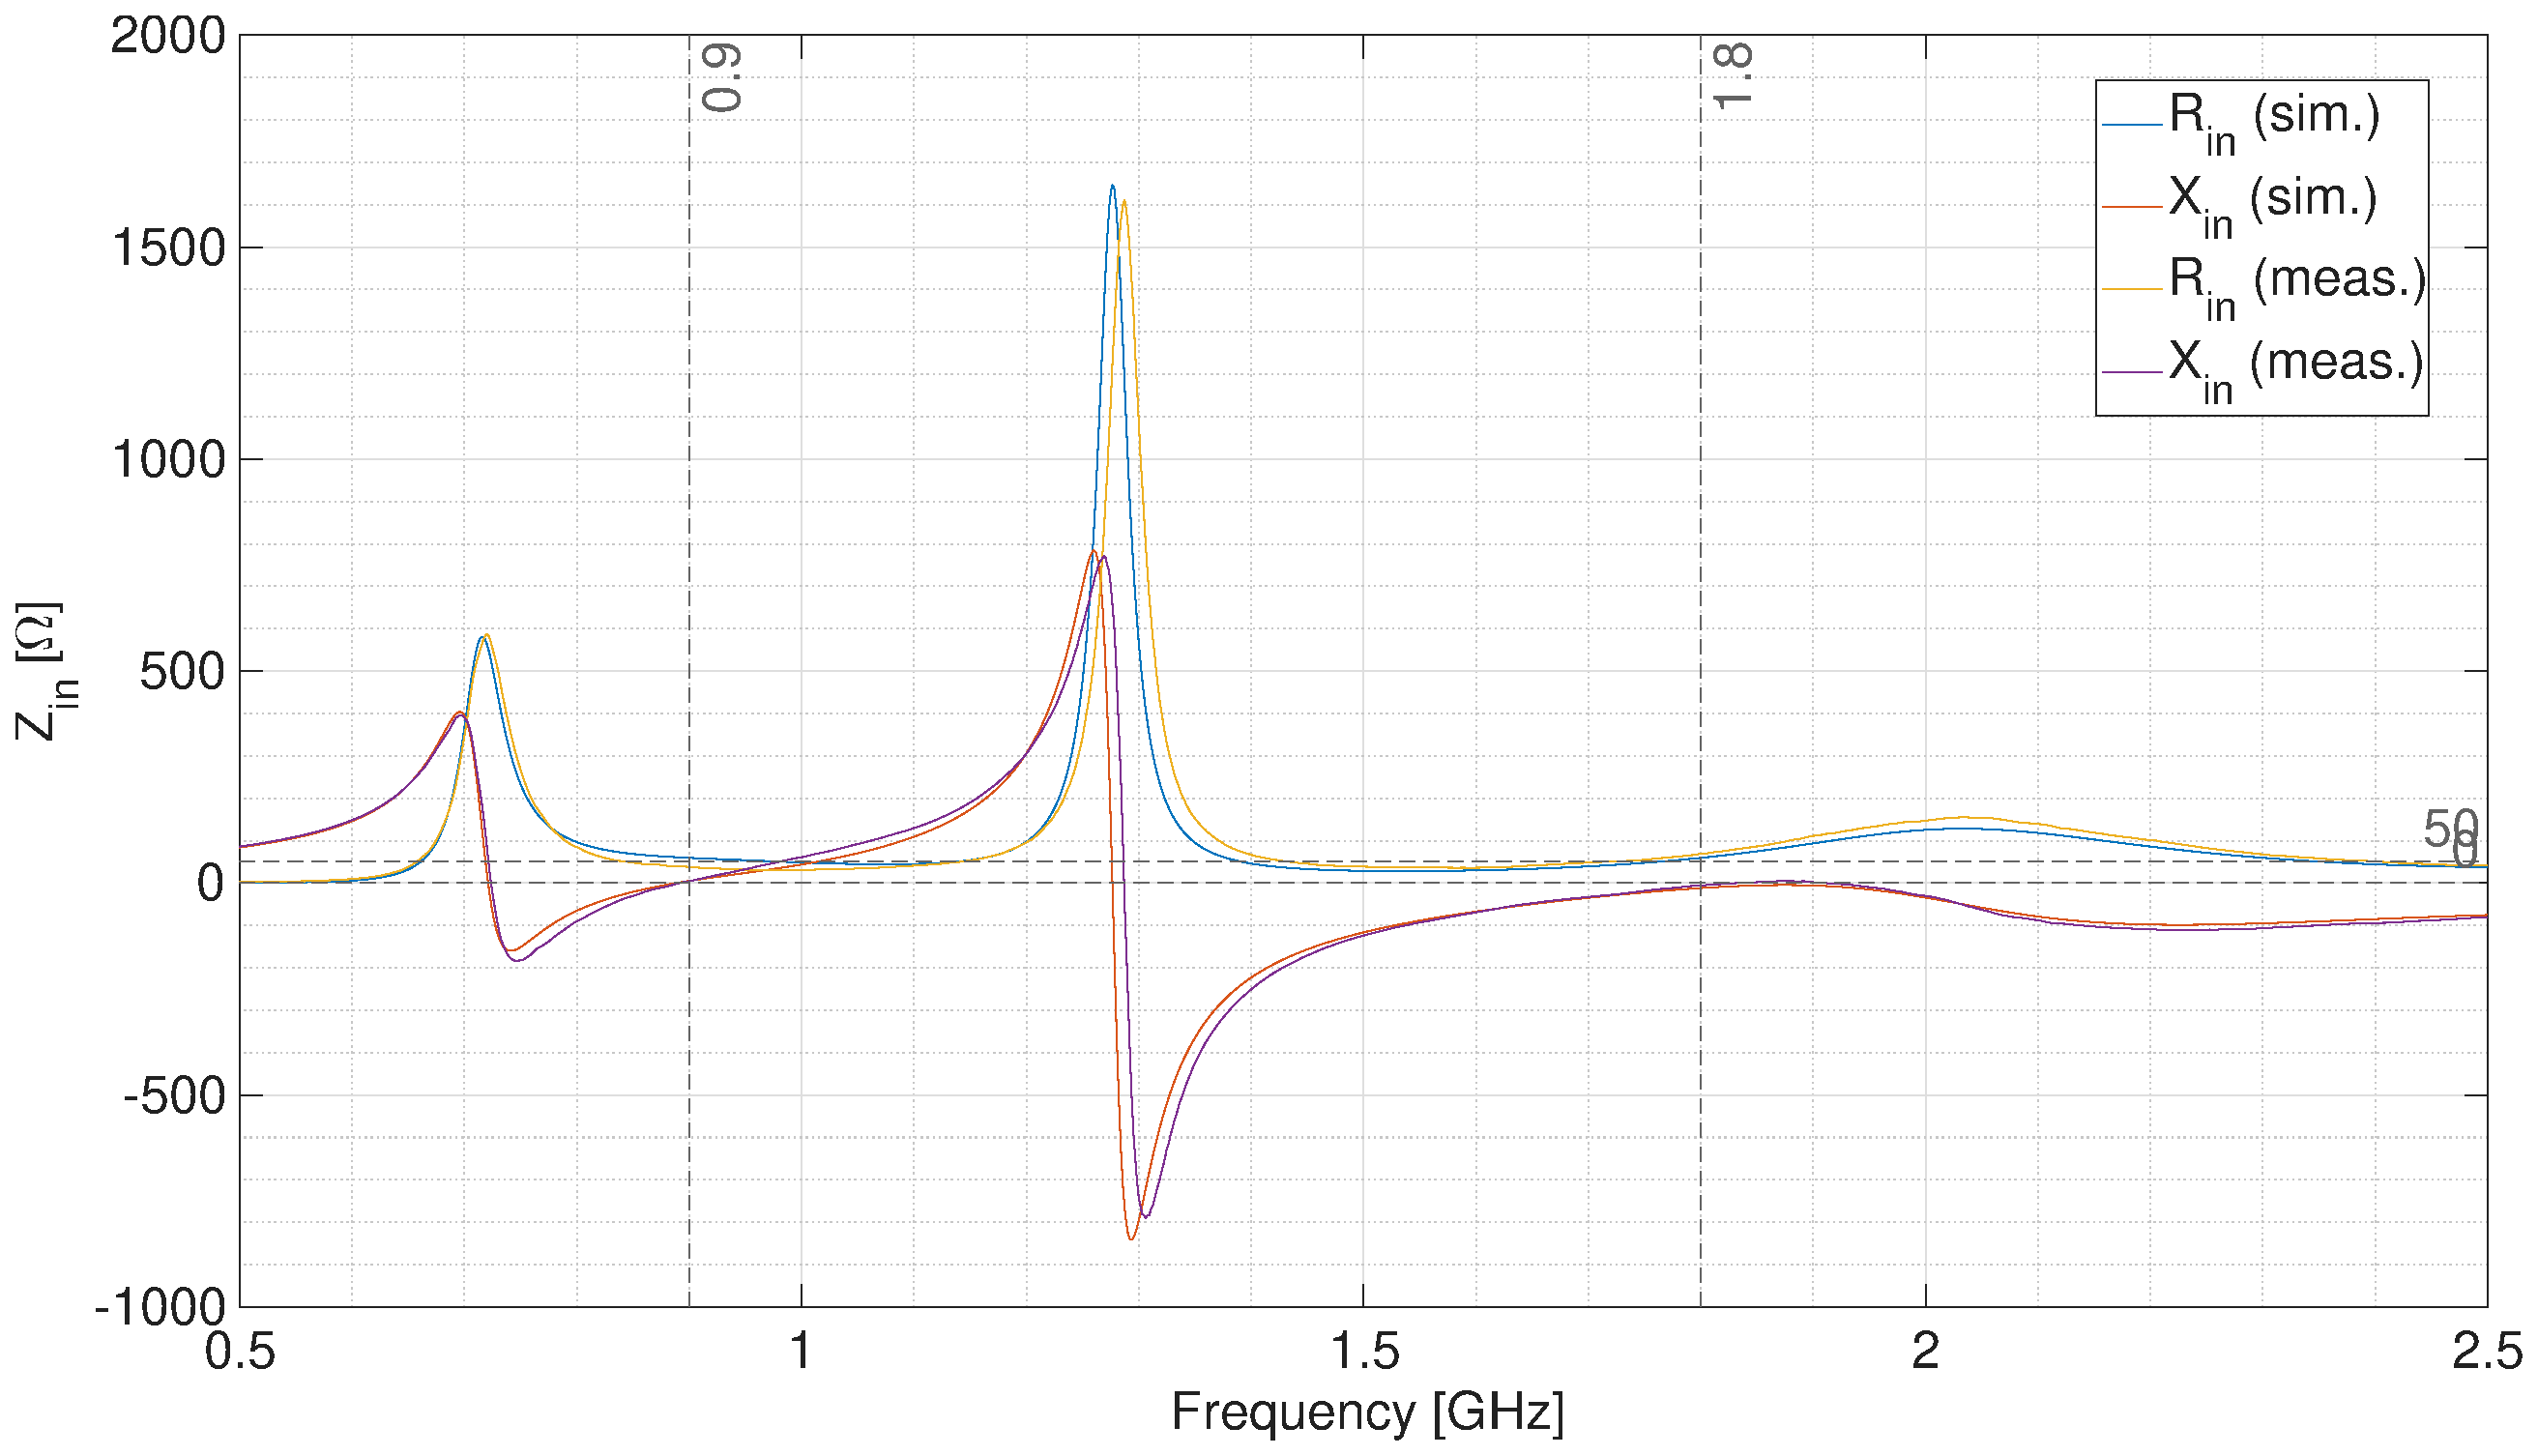
\includegraphics[width=.8\textwidth]{src/pifa-impedance.eps}
            \caption{\label{fig:pifa-impedance}PIFA: Input impedance}
        \end{figure}

        \begin{figure}[!ht]
            \centering
            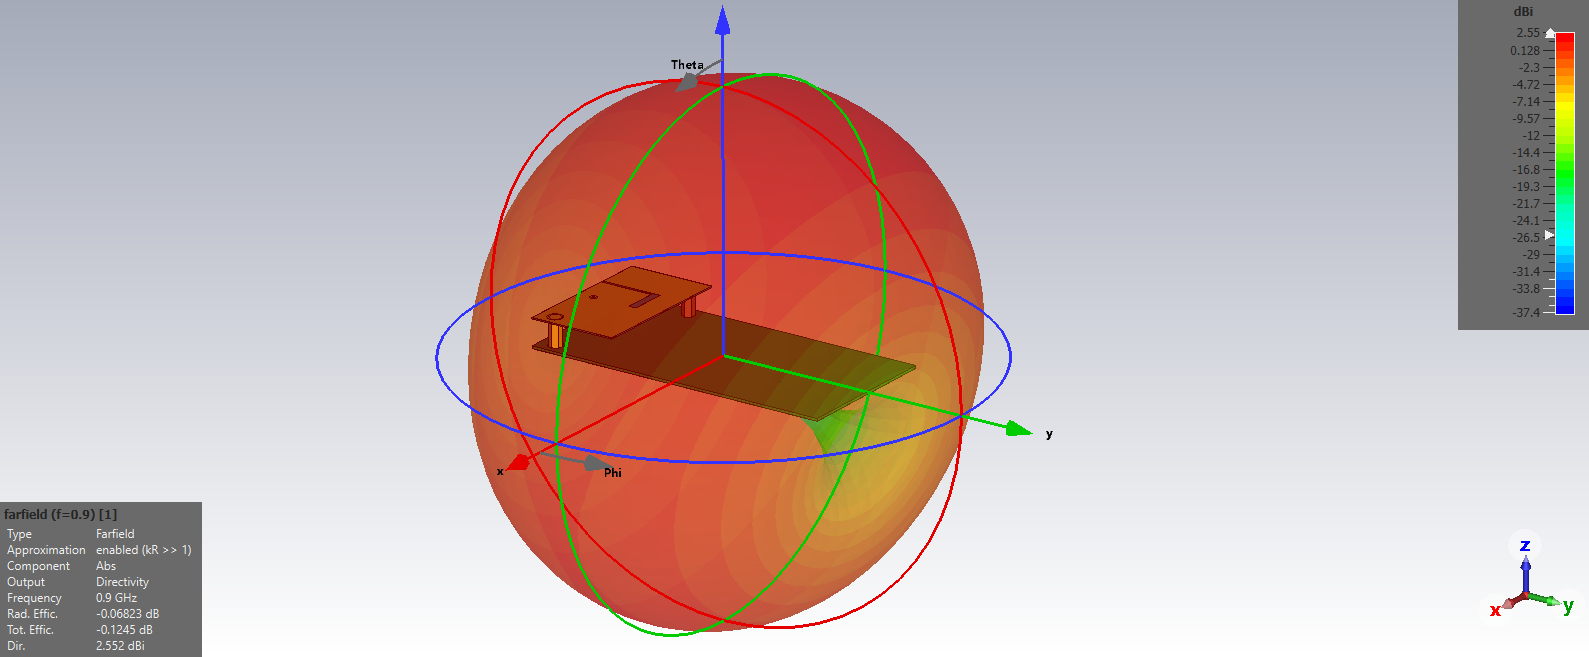
\includegraphics[width=.8\textwidth]{src/pifa-farfield-0G9Hz.png}
            \caption{\label{fig:pifa-farfield-0G9Hz}PIFA: farfield in the lower band ($0.9\, \mathrm{GHz}$)}
        \end{figure}

        \begin{figure}[!ht]
            \centering
            \begin{subfigure}{.4\textwidth}
                \centering
                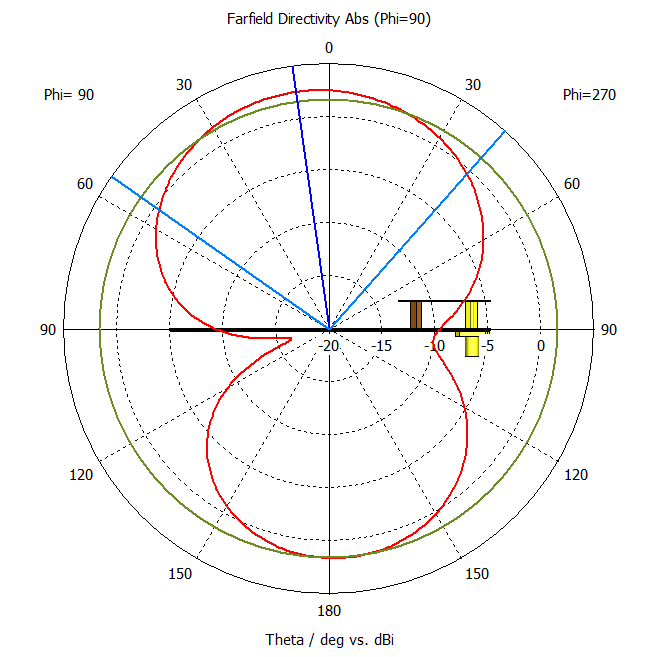
\includegraphics[width=\textwidth]{src/pifa-sim-radiation-e-0G9Hz.png}
                \caption{\label{fig:pifa-sim-radiation-e-0G9Hz}Simulation}
            \end{subfigure}
            ~
            \begin{subfigure}{.4\textwidth}
                \centering
                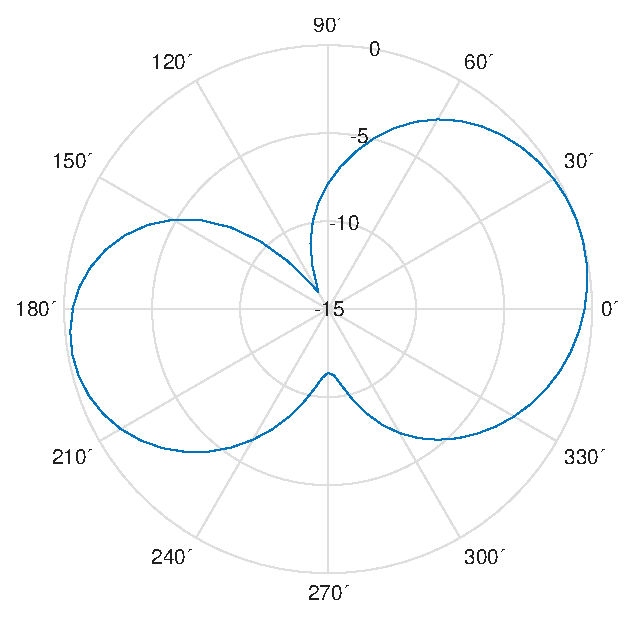
\includegraphics[width=\textwidth]{src/pifa-meas-radiation-e-0G9Hz.eps}
                \caption{\label{fig:pifa-meas-radiation-e-0G9Hz}Measurement}
            \end{subfigure}
            \caption{\label{fig:pifa-radiation-e-0G9Hz}PIFA: $E$-cut of the radiation pattern in the lower band ($0.9\, \mathrm{GHz}$)}
        \end{figure}

\newpage
        \begin{figure}[!ht]
            \centering
            \begin{subfigure}{.4\textwidth}
                \centering
                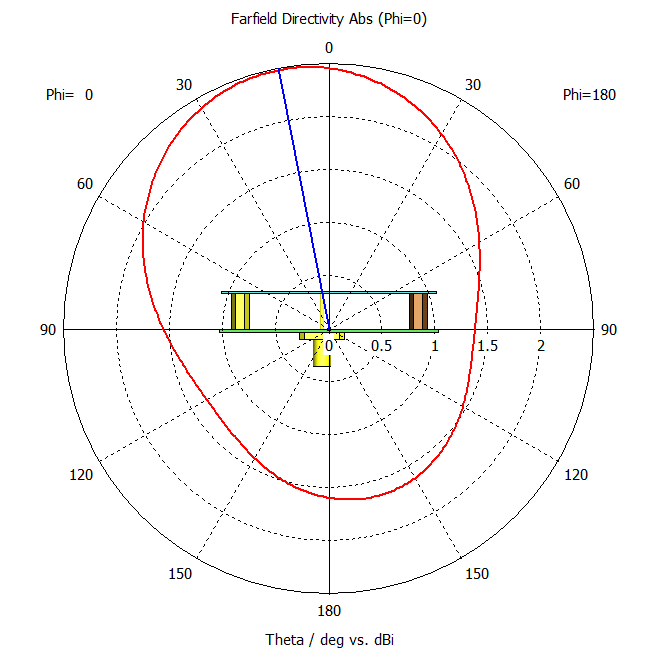
\includegraphics[width=\textwidth]{src/pifa-sim-radiation-h-0G9Hz.png}
                \caption{\label{fig:pifa-sim-radiation-h-0G9Hz}Simulation}
            \end{subfigure}
            ~
            \begin{subfigure}{.4\textwidth}
                \centering
                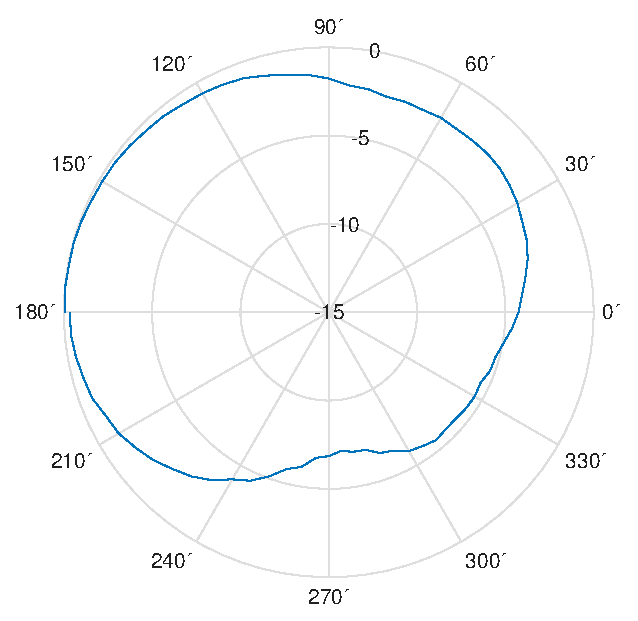
\includegraphics[width=\textwidth]{src/pifa-meas-radiation-h-0G9Hz.eps}
                \caption{\label{fig:pifa-meas-radiation-h-0G9Hz}Measurement}
            \end{subfigure}
            \caption{\label{fig:pifa-radiation-h-0G9Hz}PIFA: $H$-cut of the radiation pattern in the lower band ($0.9\, \mathrm{GHz}$)}
        \end{figure}

        \begin{figure}[!ht]
            \centering
            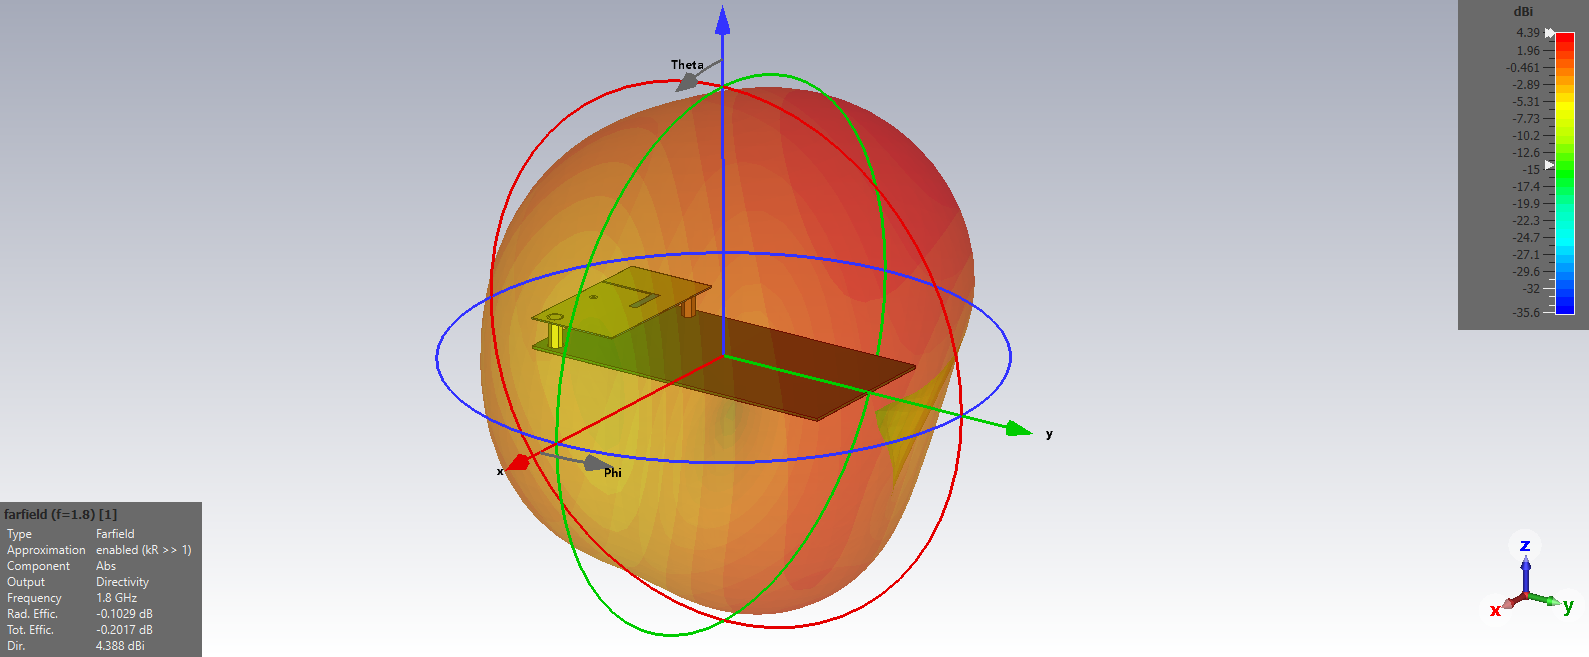
\includegraphics[width=.8\textwidth]{src/pifa-farfield-1G8Hz.png}
            \caption{\label{fig:pifa-farfield-1G8Hz}PIFA: farfield in the upper band ($1.8\, \mathrm{GHz}$)}
        \end{figure}

        \begin{figure}[!ht]
            \centering
            \begin{subfigure}{.4\textwidth}
                \centering
                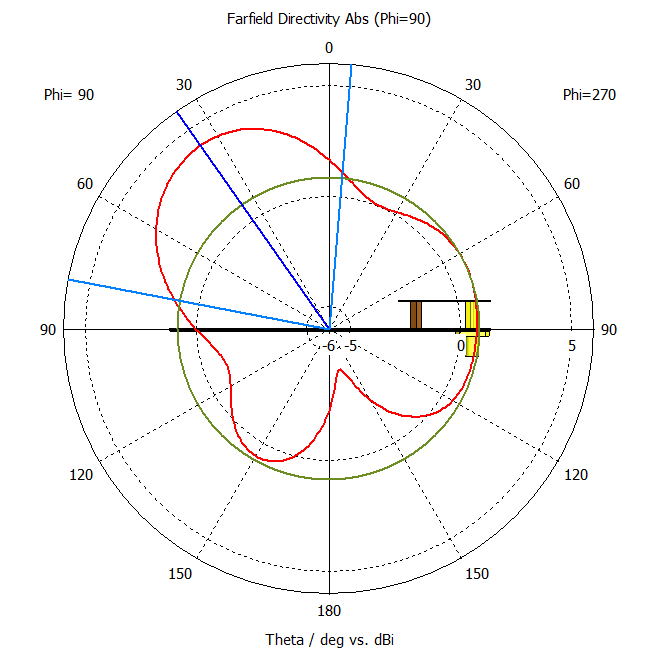
\includegraphics[width=\textwidth]{src/pifa-sim-radiation-e-1G8Hz.png}
                \caption{\label{fig:pifa-sim-radiation-e-1G8Hz}Simulation}
            \end{subfigure}
            ~
            \begin{subfigure}{.4\textwidth}
                \centering
                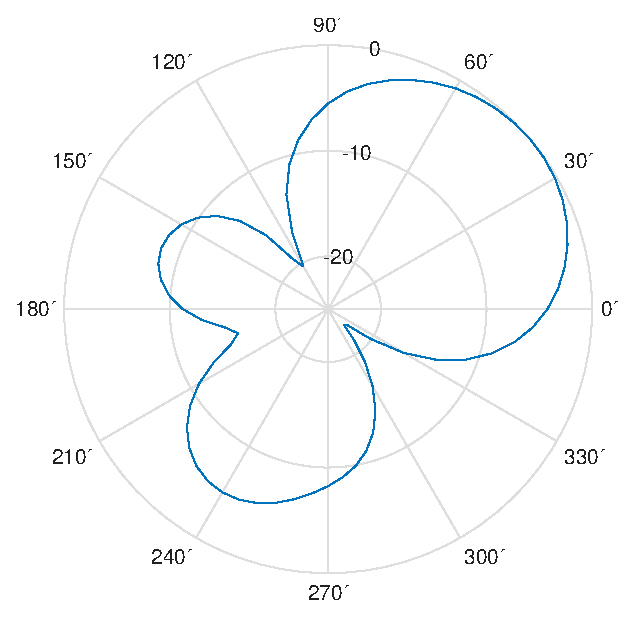
\includegraphics[width=\textwidth]{src/pifa-meas-radiation-e-1G8Hz.eps}
                \caption{\label{fig:pifa-meas-radiation-e-1G8Hz}Measurement}
            \end{subfigure}
            \caption{\label{fig:pifa-radiation-e-1G8Hz}PIFA: $E$-cut of the radiation pattern in the upper band ($1.8\, \mathrm{GHz}$)}
        \end{figure}

\newpage
        \begin{figure}[!ht]
            \centering
            \begin{subfigure}{.4\textwidth}
                \centering
                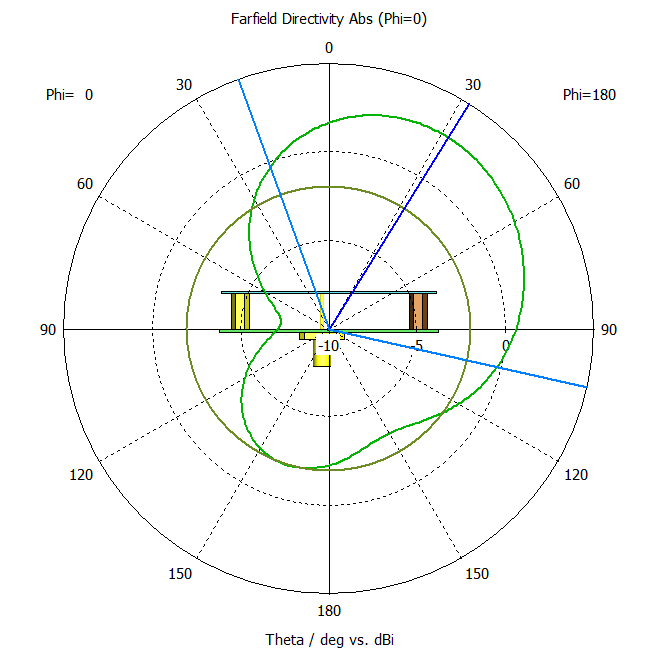
\includegraphics[width=\textwidth]{src/pifa-sim-radiation-h-1G8Hz.png}
                \caption{\label{fig:pifa-sim-radiation-h-1G8Hz}Simulation}
            \end{subfigure}
            ~
            \begin{subfigure}{.4\textwidth}
                \centering
                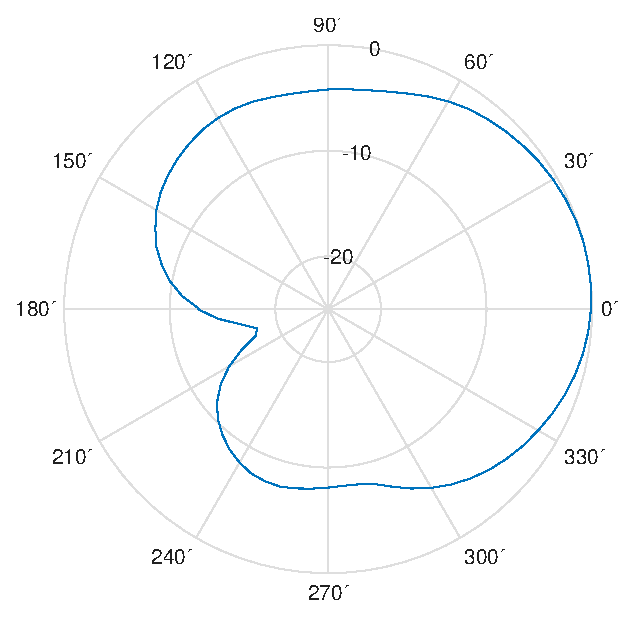
\includegraphics[width=\textwidth]{src/pifa-meas-radiation-h-1G8Hz.eps}
                \caption{\label{fig:pifa-meas-radiation-h-1G8Hz}Measurement}
            \end{subfigure}
            \caption{\label{fig:pifa-radiation-h-1G8Hz}PIFA: $H$-cut of the radiation pattern in the upper band ($1.8\, \mathrm{GHz}$)}
        \end{figure}

\newpage
        \paragraph{Lambda-tenth monopole} The antenna was designed to the fulfilment of the assignment. This can be seen in Figure~\ref{fig:lambda-tenth-reflection-linear} where the magnitude of the reflection coefficient clearly reaches the expected values around both resonant frequencies. Furthermore, the complex reflection coefficient is shown using a Smith chart in Figure~\ref{fig:lambda-tenth-reflection-smith} and the input impedance is plotted by parts in Figure~\ref{fig:lambda-tenth-impedance}. The radiation properties are conveyed both in 3D and 2D. Figure~\ref{fig:lambda-tenth-farfield} shows the 3D farfield pattern. The radiation patterns can also be inspected in cuts through the $E$- and $H$-plane in Figure~\ref{fig:lambda-tenth-radiation}.
        
        \begin{figure}[!ht]
            \centering
            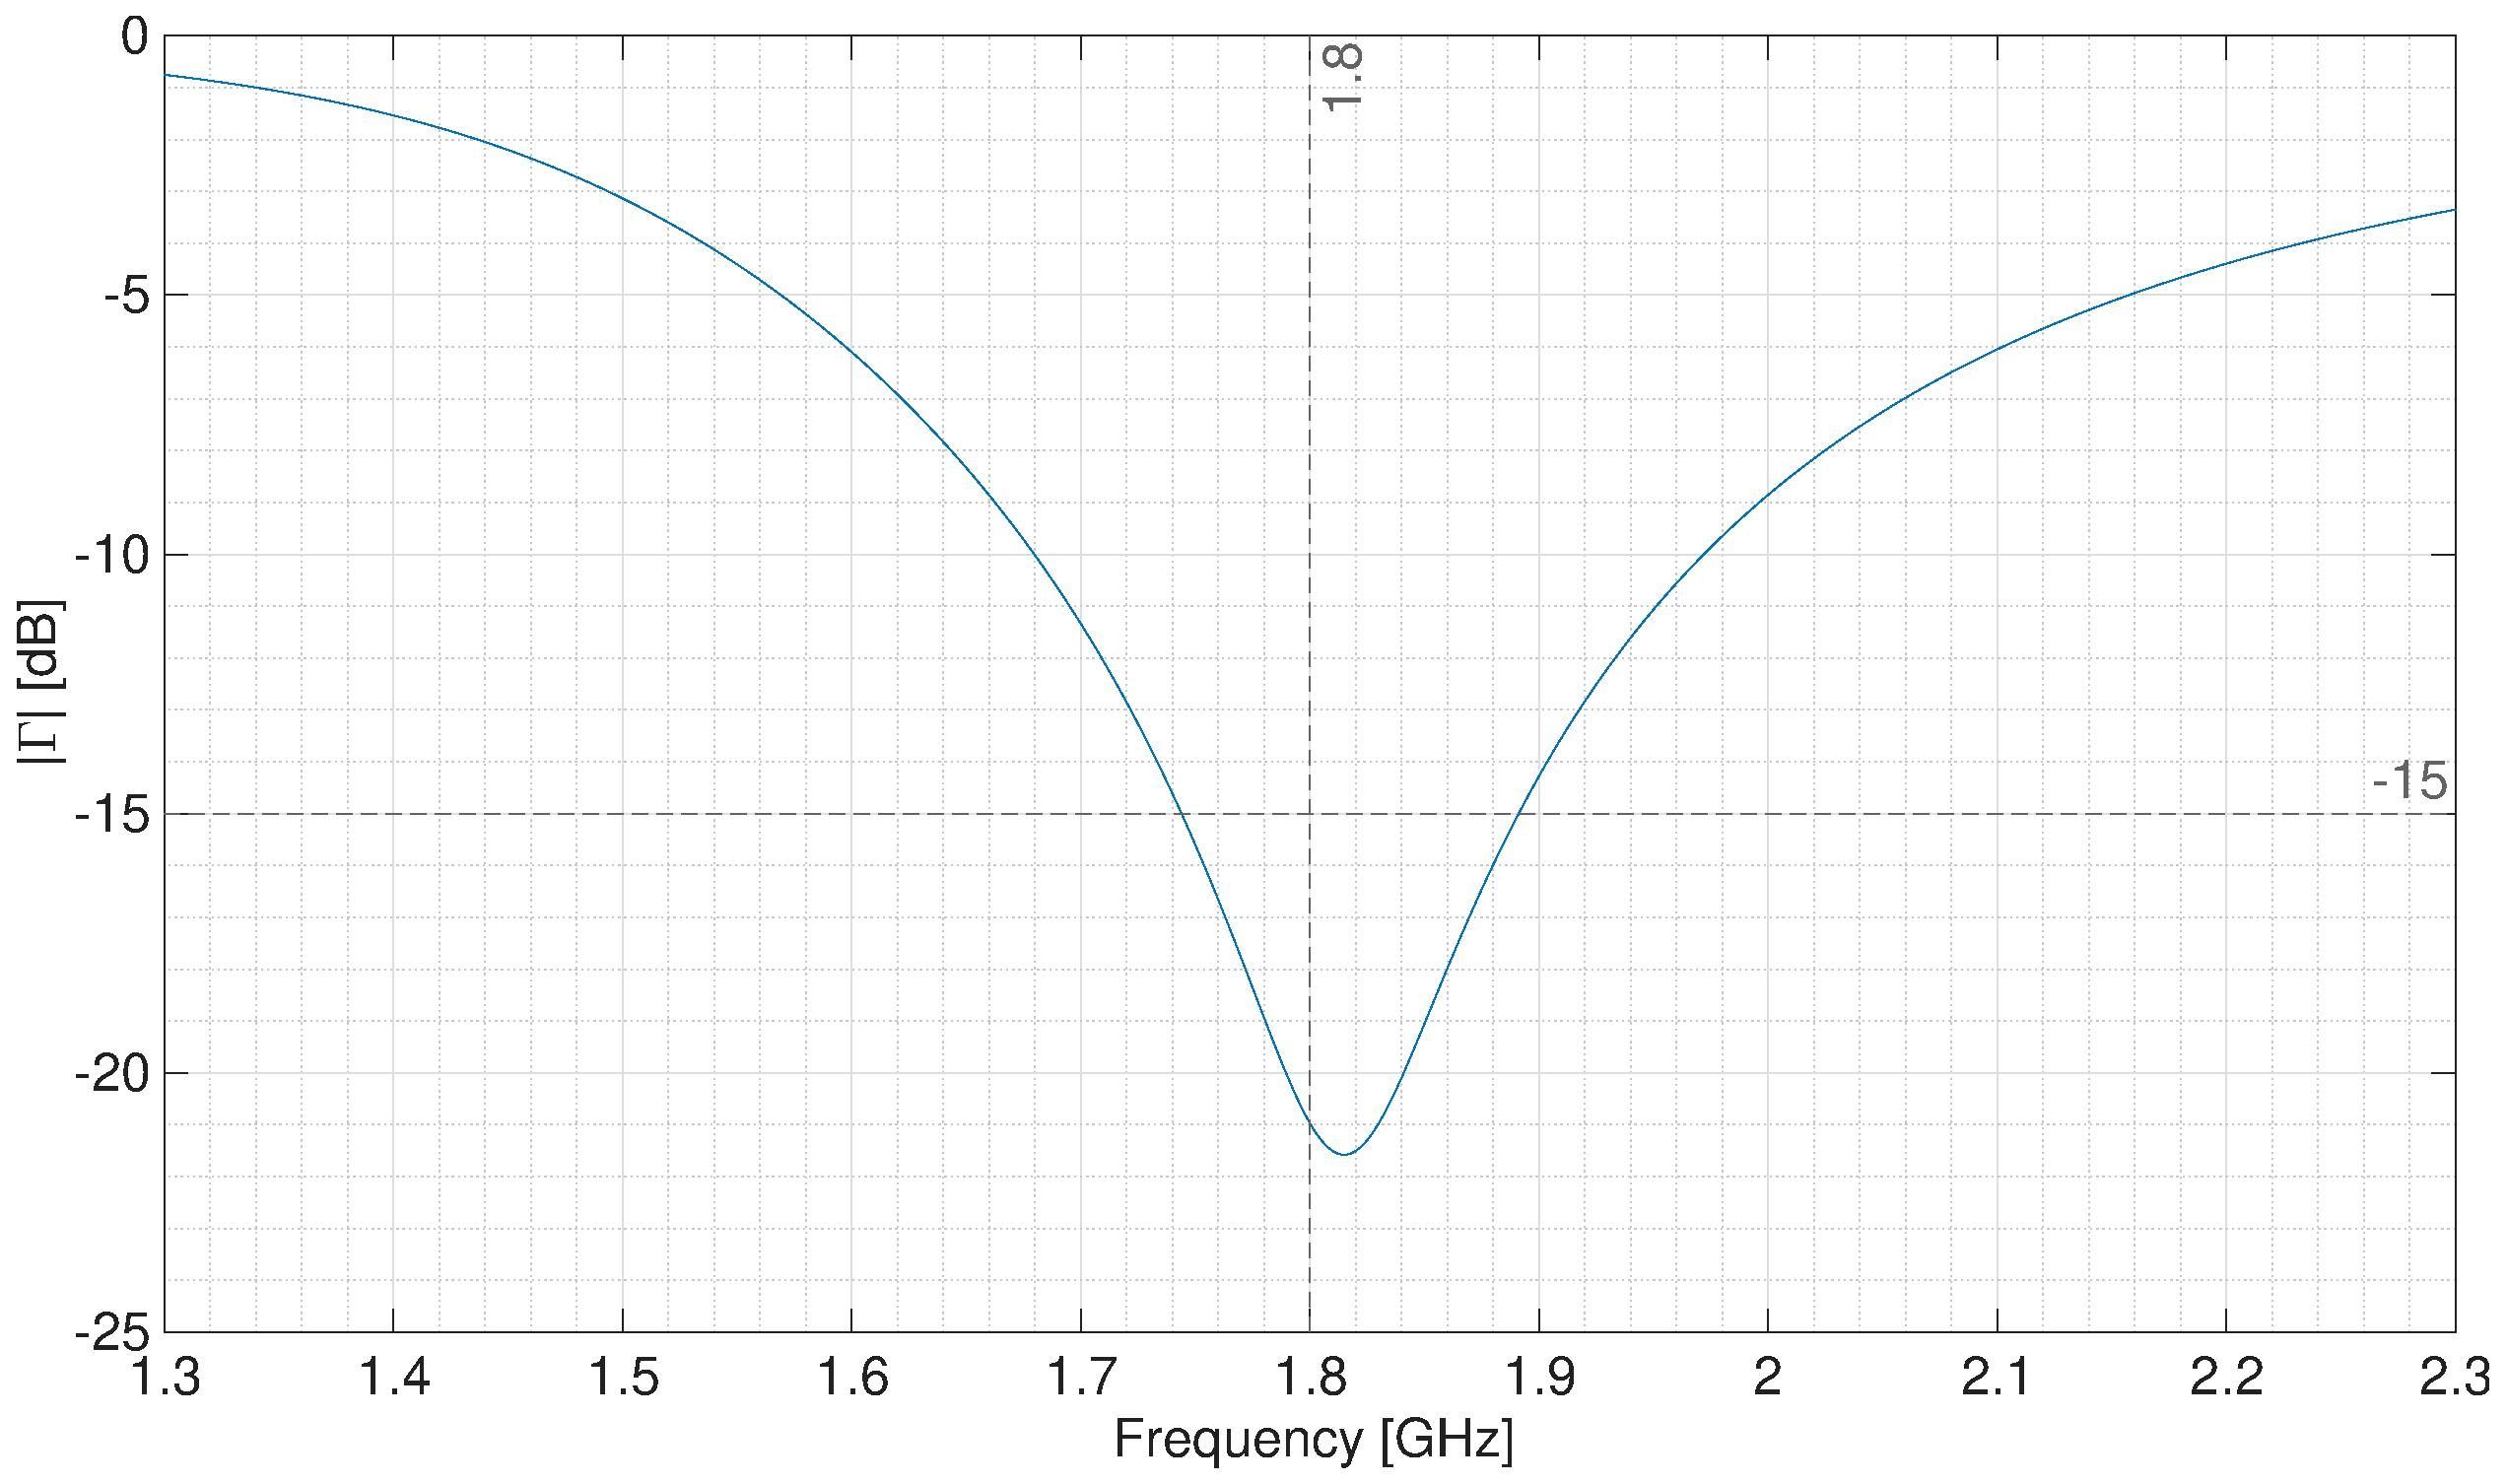
\includegraphics[width=.8\textwidth]{src/lambda-tenth-reflection-linear.eps}
            \caption{\label{fig:lambda-tenth-reflection-linear}Lambda-tenth monopole: Reflection coefficient in the linear scale}
        \end{figure}
        
        \begin{figure}[!ht]
            \centering
            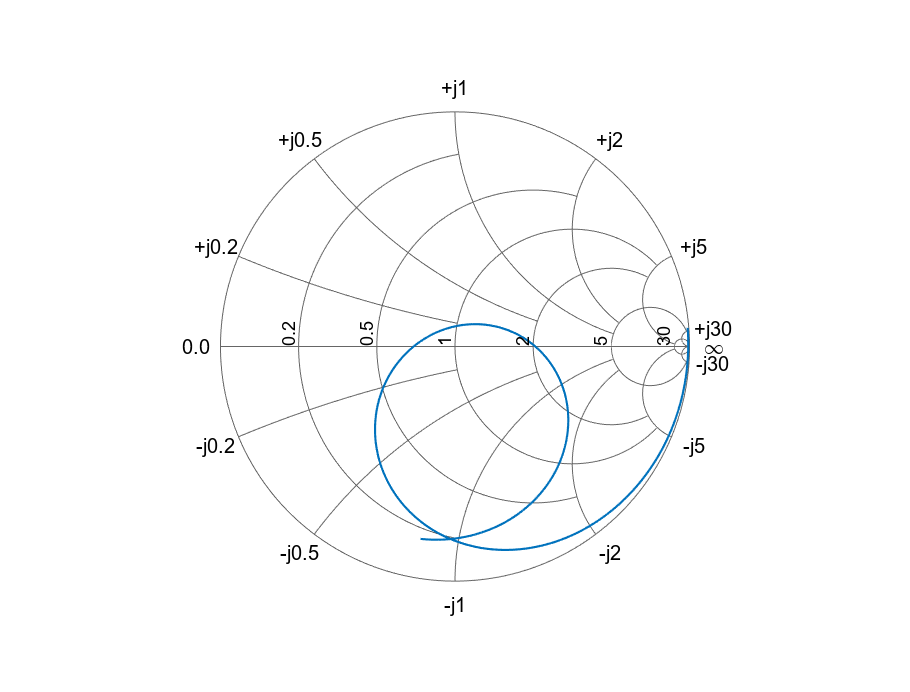
\includegraphics[width=.8\textwidth]{src/lambda-tenth-reflection-smith.eps}
            \caption{\label{fig:lambda-tenth-reflection-smith}Lambda-tenth monopole: Reflection coefficient in the Smith chart}
        \end{figure}

        \begin{figure}[!ht]
            \centering
            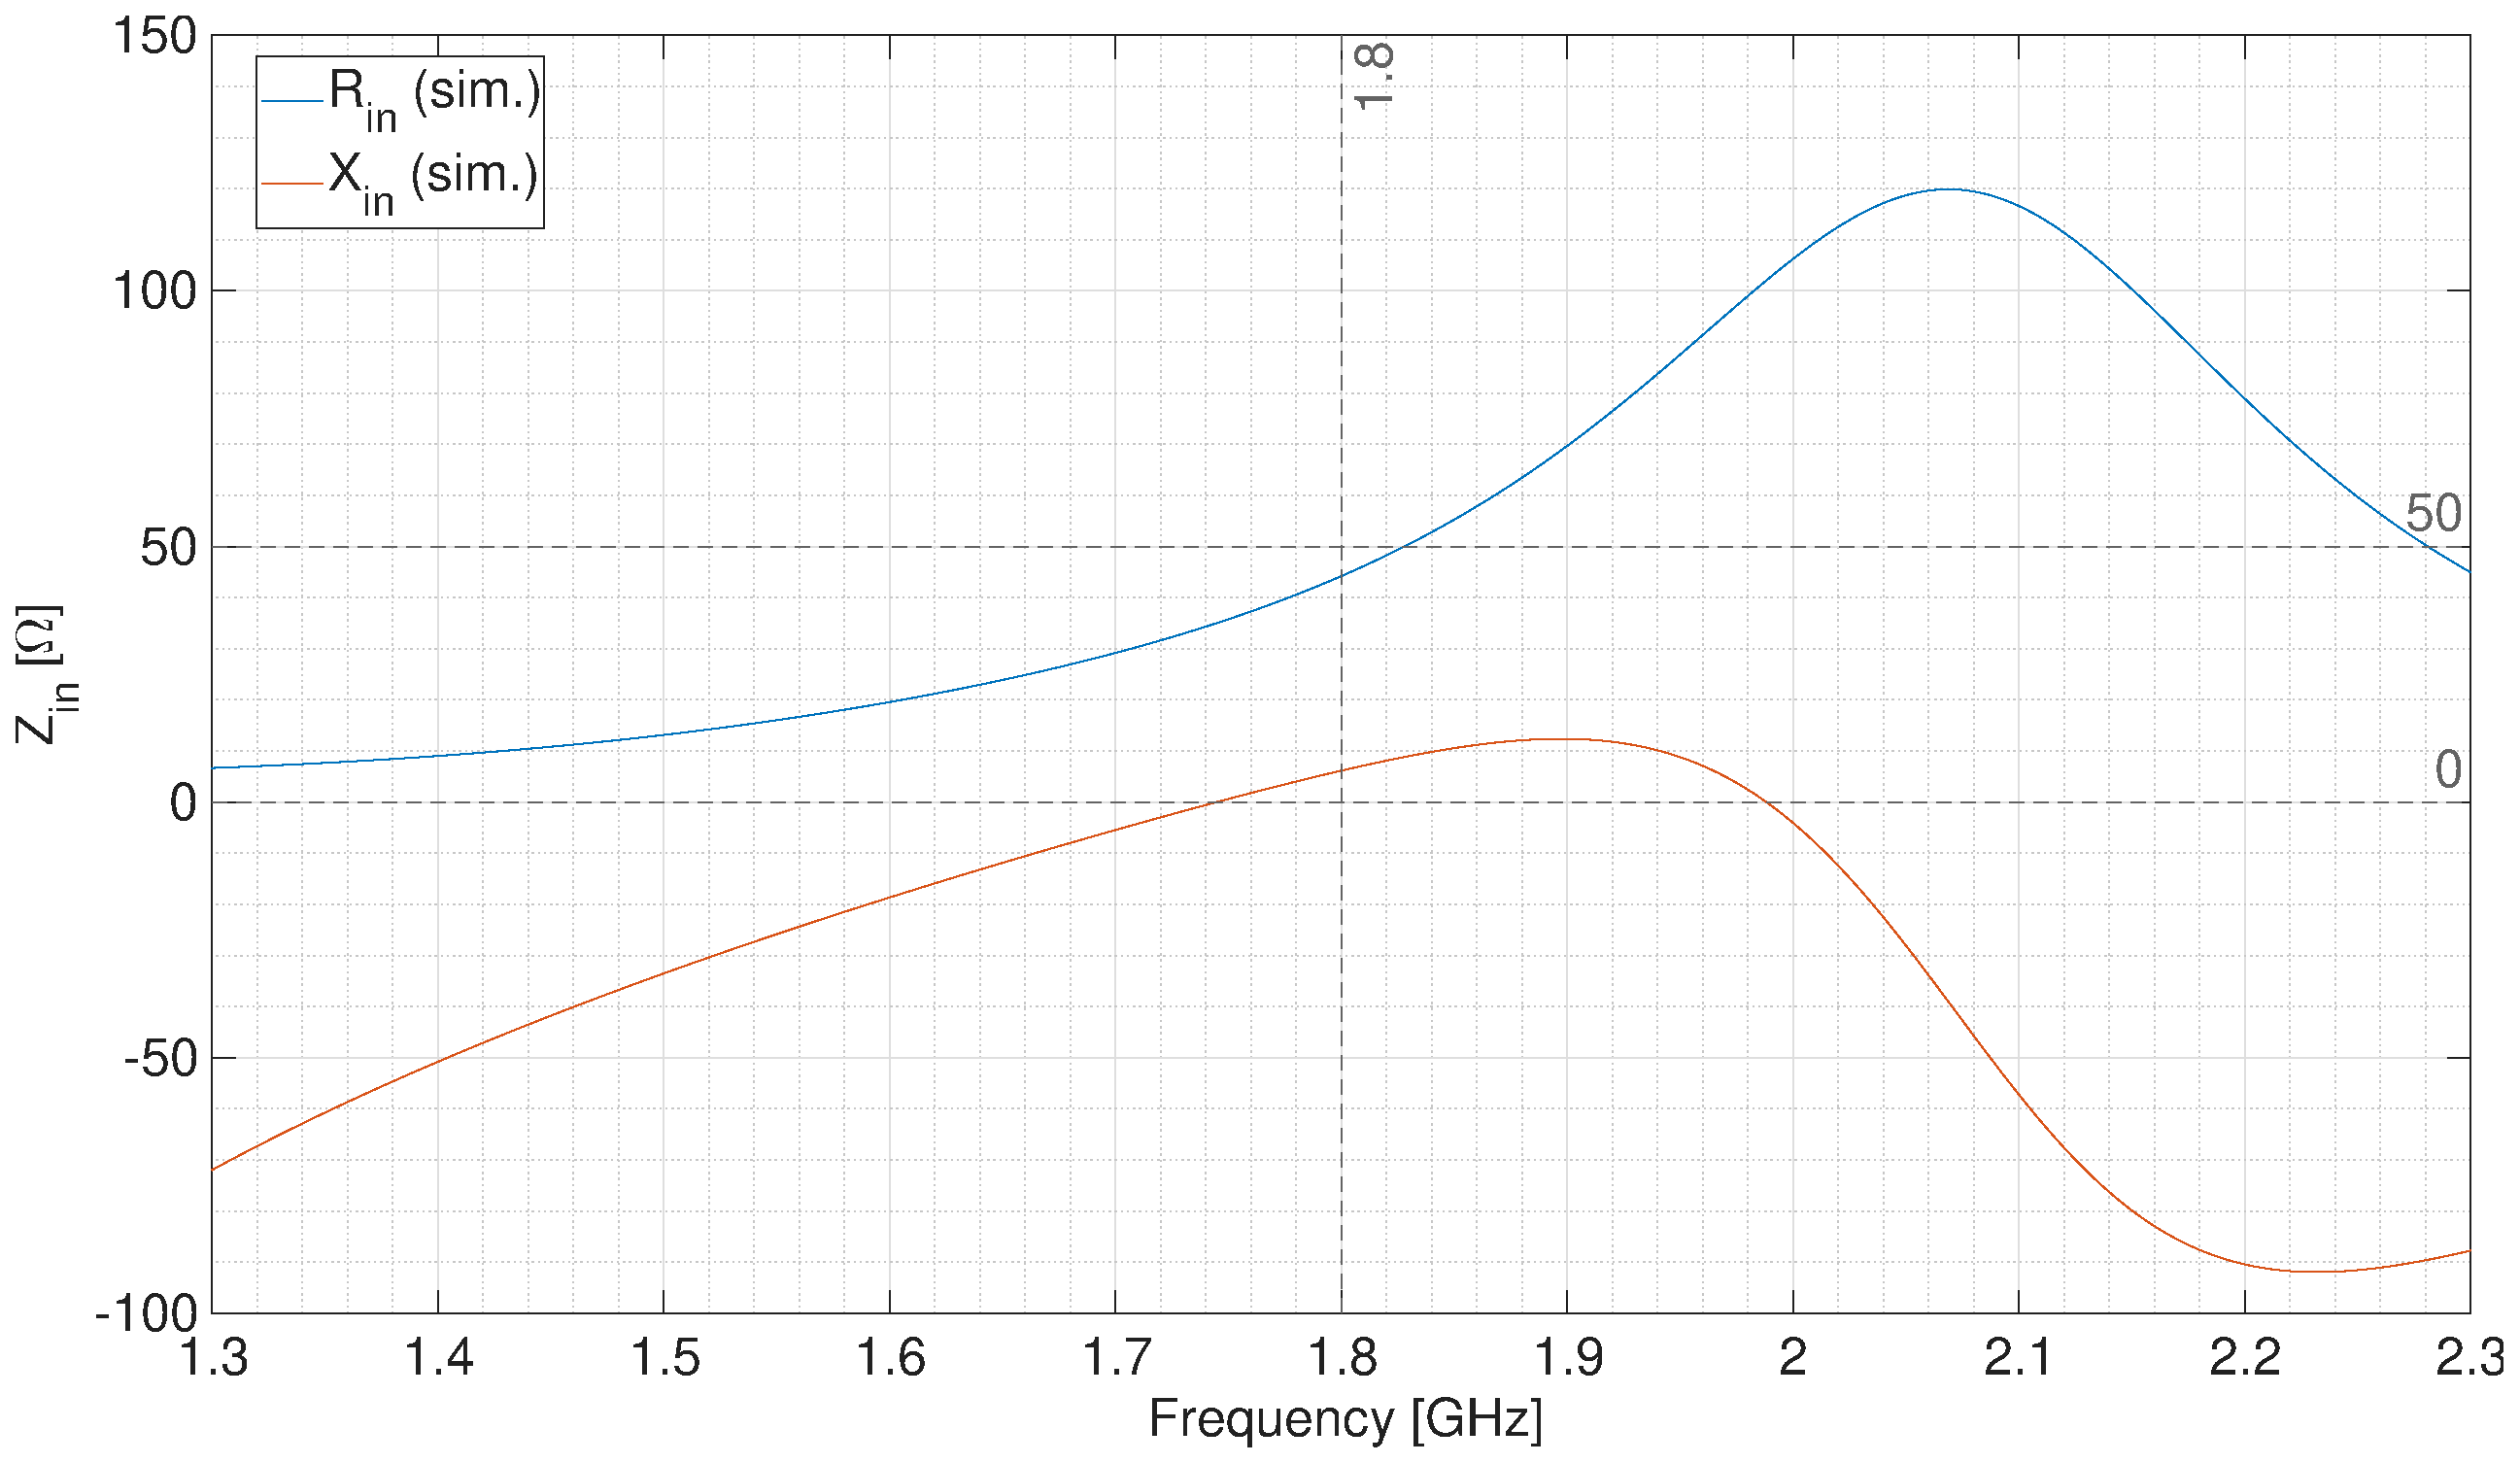
\includegraphics[width=.8\textwidth]{src/lambda-tenth-impedance.eps}
            \caption{\label{fig:lambda-tenth-impedance}Lambda-tenth monopole: Input impedance}
        \end{figure}

\newpage
        \begin{figure}[!ht]
            \centering
            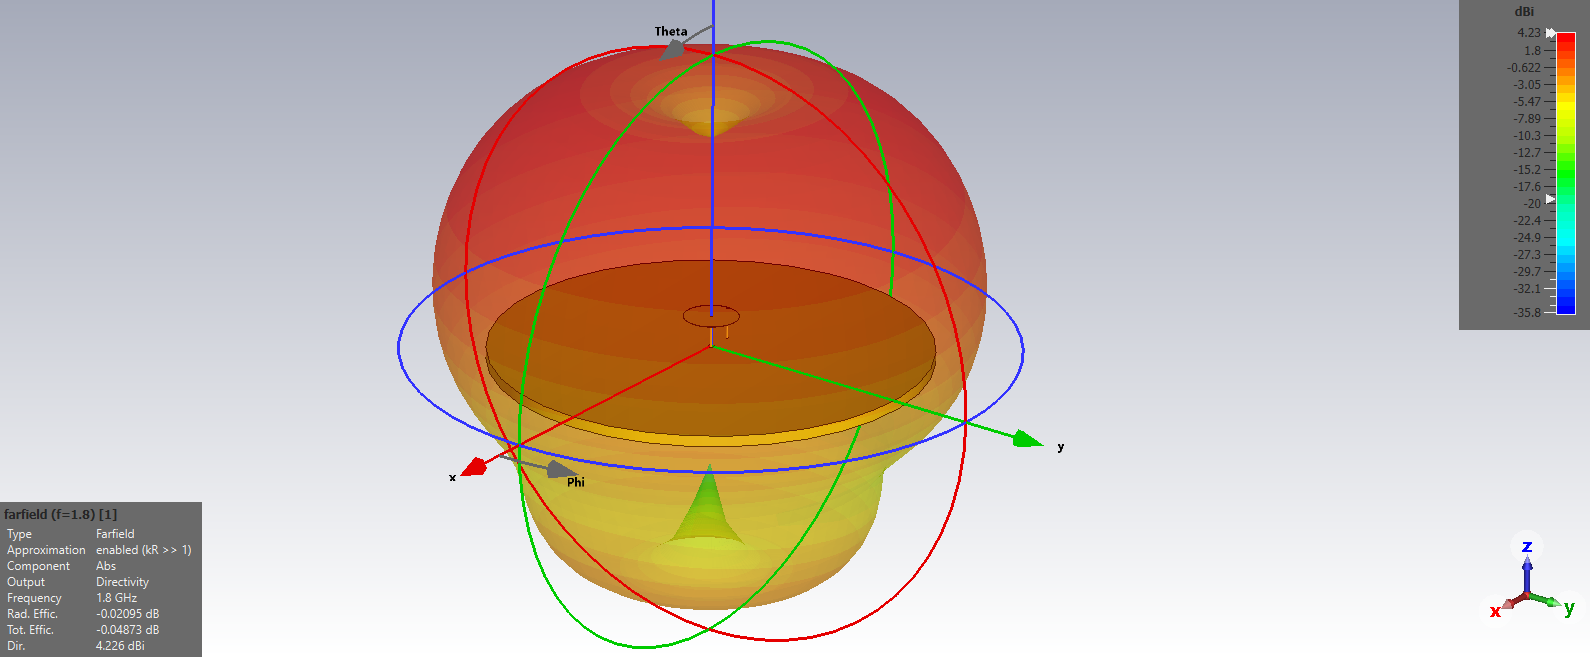
\includegraphics[width=.8\textwidth]{src/lambda-tenth-farfield.png}
            \caption{\label{fig:lambda-tenth-farfield}Lambda-tenth monopole: farfield}
        \end{figure}

        \begin{figure}[!ht]
            \centering
            \begin{subfigure}{.4\textwidth}
                \centering
                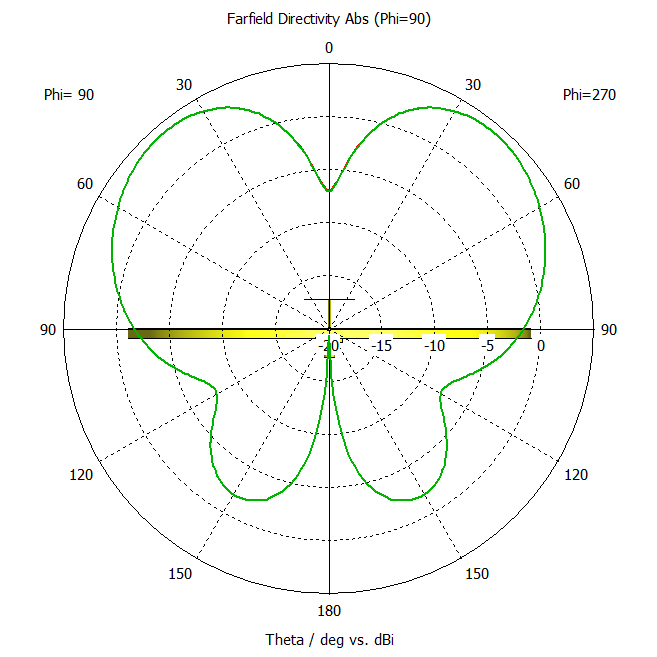
\includegraphics[width=\textwidth]{src/lambda-tenth-radiation-e.png}
                \caption{\label{fig:lambda-tenth-radiation-e}$E$-plane}
            \end{subfigure}
            ~
            \begin{subfigure}{.4\textwidth}
                \centering
                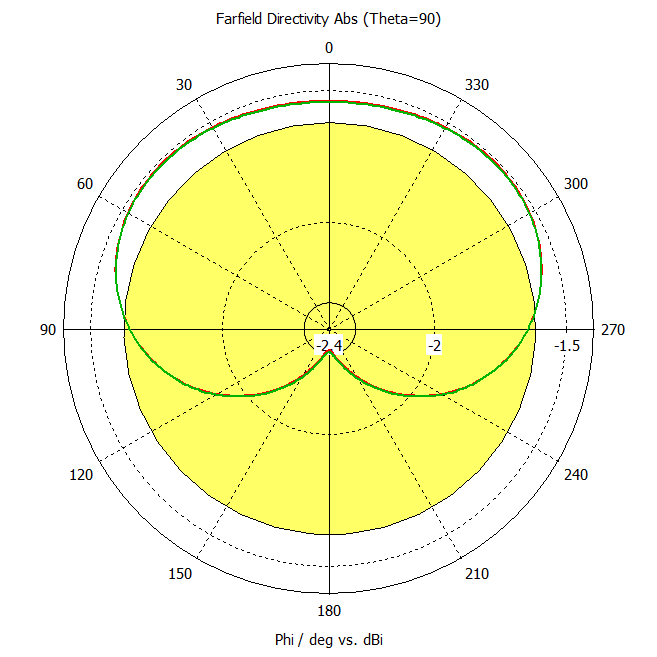
\includegraphics[width=\textwidth]{src/lambda-tenth-radiation-h.png}
                \caption{\label{fig:lambda-tenth-sim-radiation-h}$H$-plane}
            \end{subfigure}
            \caption{\label{fig:lambda-tenth-radiation}Lambda-tenth monopole: radiation pattern cuts}
        \end{figure}

\newpage
        \paragraph{Lambda-twentieth monopole} The antenna was designed to the fulfilment of the assignment. This can be seen in Figure~\ref{fig:lambda-twentieth-reflection-linear} where the magnitude of the reflection coefficient clearly reaches the expected values around both resonant frequencies. Furthermore, the complex reflection coefficient is shown using a Smith chart in Figure~\ref{fig:lambda-twentieth-reflection-smith} and the input impedance is plotted by parts in Figure~\ref{fig:lambda-twentieth-impedance}. The radiation properties are conveyed both in 3D and 2D. Figure~\ref{fig:lambda-twentieth-farfield} shows the 3D farfield pattern. The radiation patterns can also be inspected in cuts through the $E$- and $H$-plane in Figure~\ref{fig:lambda-twentieth-radiation}.
        
        \begin{figure}[!ht]
            \centering
            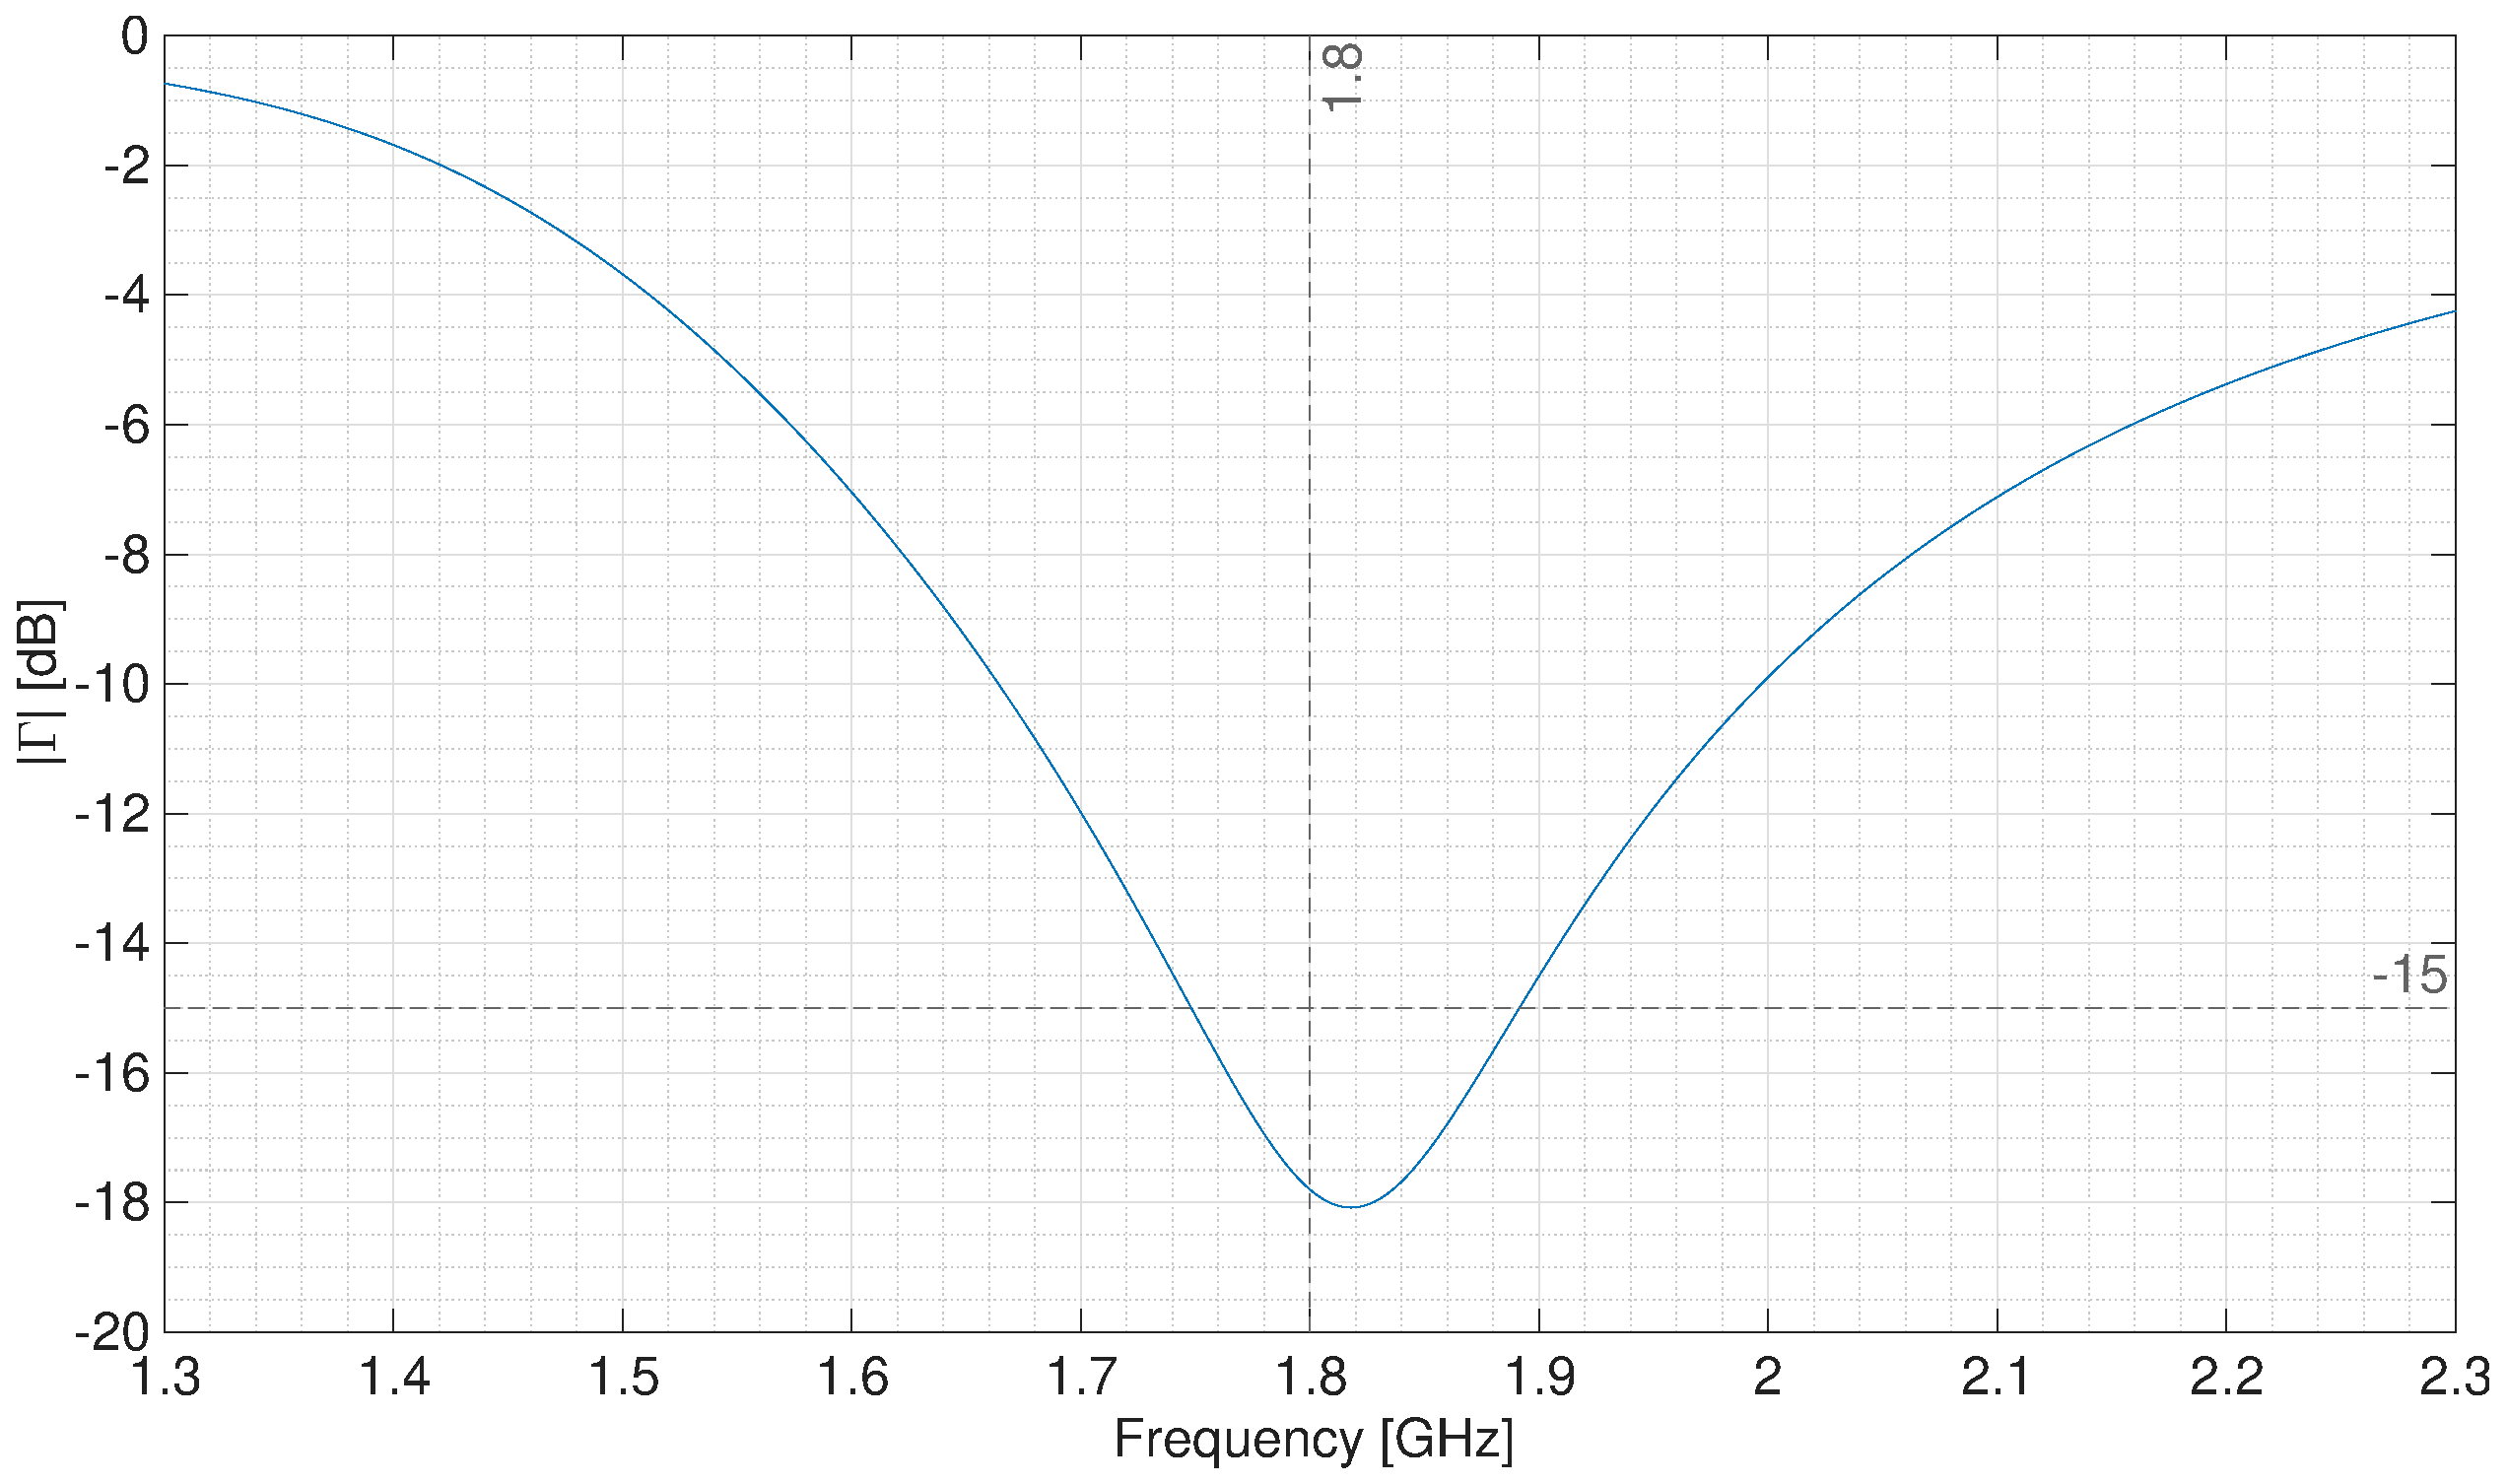
\includegraphics[width=.8\textwidth]{src/lambda-twentieth-reflection-linear.eps}
            \caption{\label{fig:lambda-twentieth-reflection-linear}Lambda-twentieth monopole: Reflection coefficient in the linear scale}
        \end{figure}
        
        \begin{figure}[!ht]
            \centering
            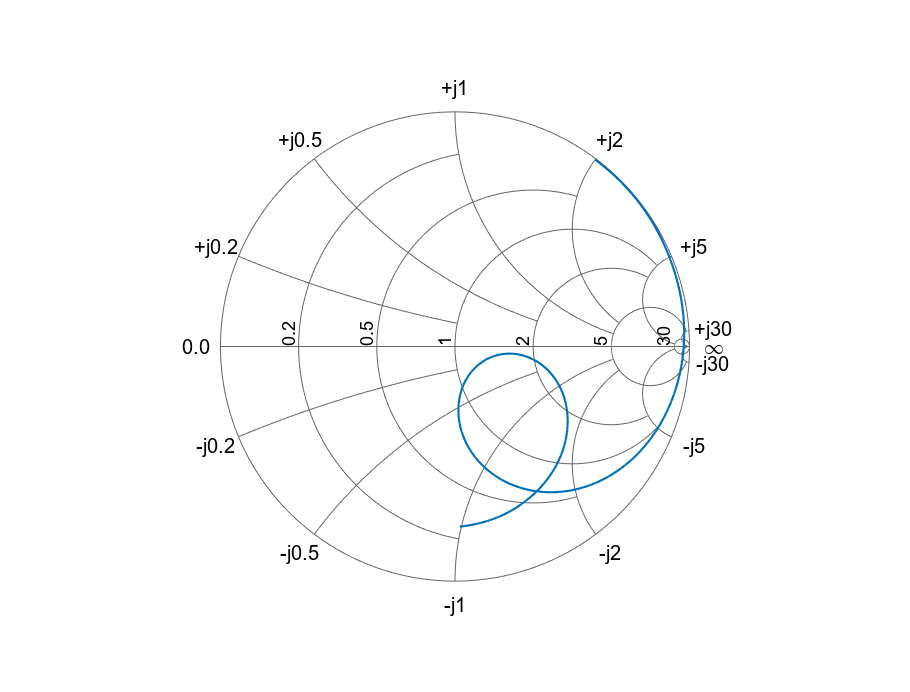
\includegraphics[width=.8\textwidth]{src/lambda-twentieth-reflection-smith.eps}
            \caption{\label{fig:lambda-twentieth-reflection-smith}Lambda-twentieth monopole: Reflection coefficient in the Smith chart}
        \end{figure}

        \begin{figure}[!ht]
            \centering
            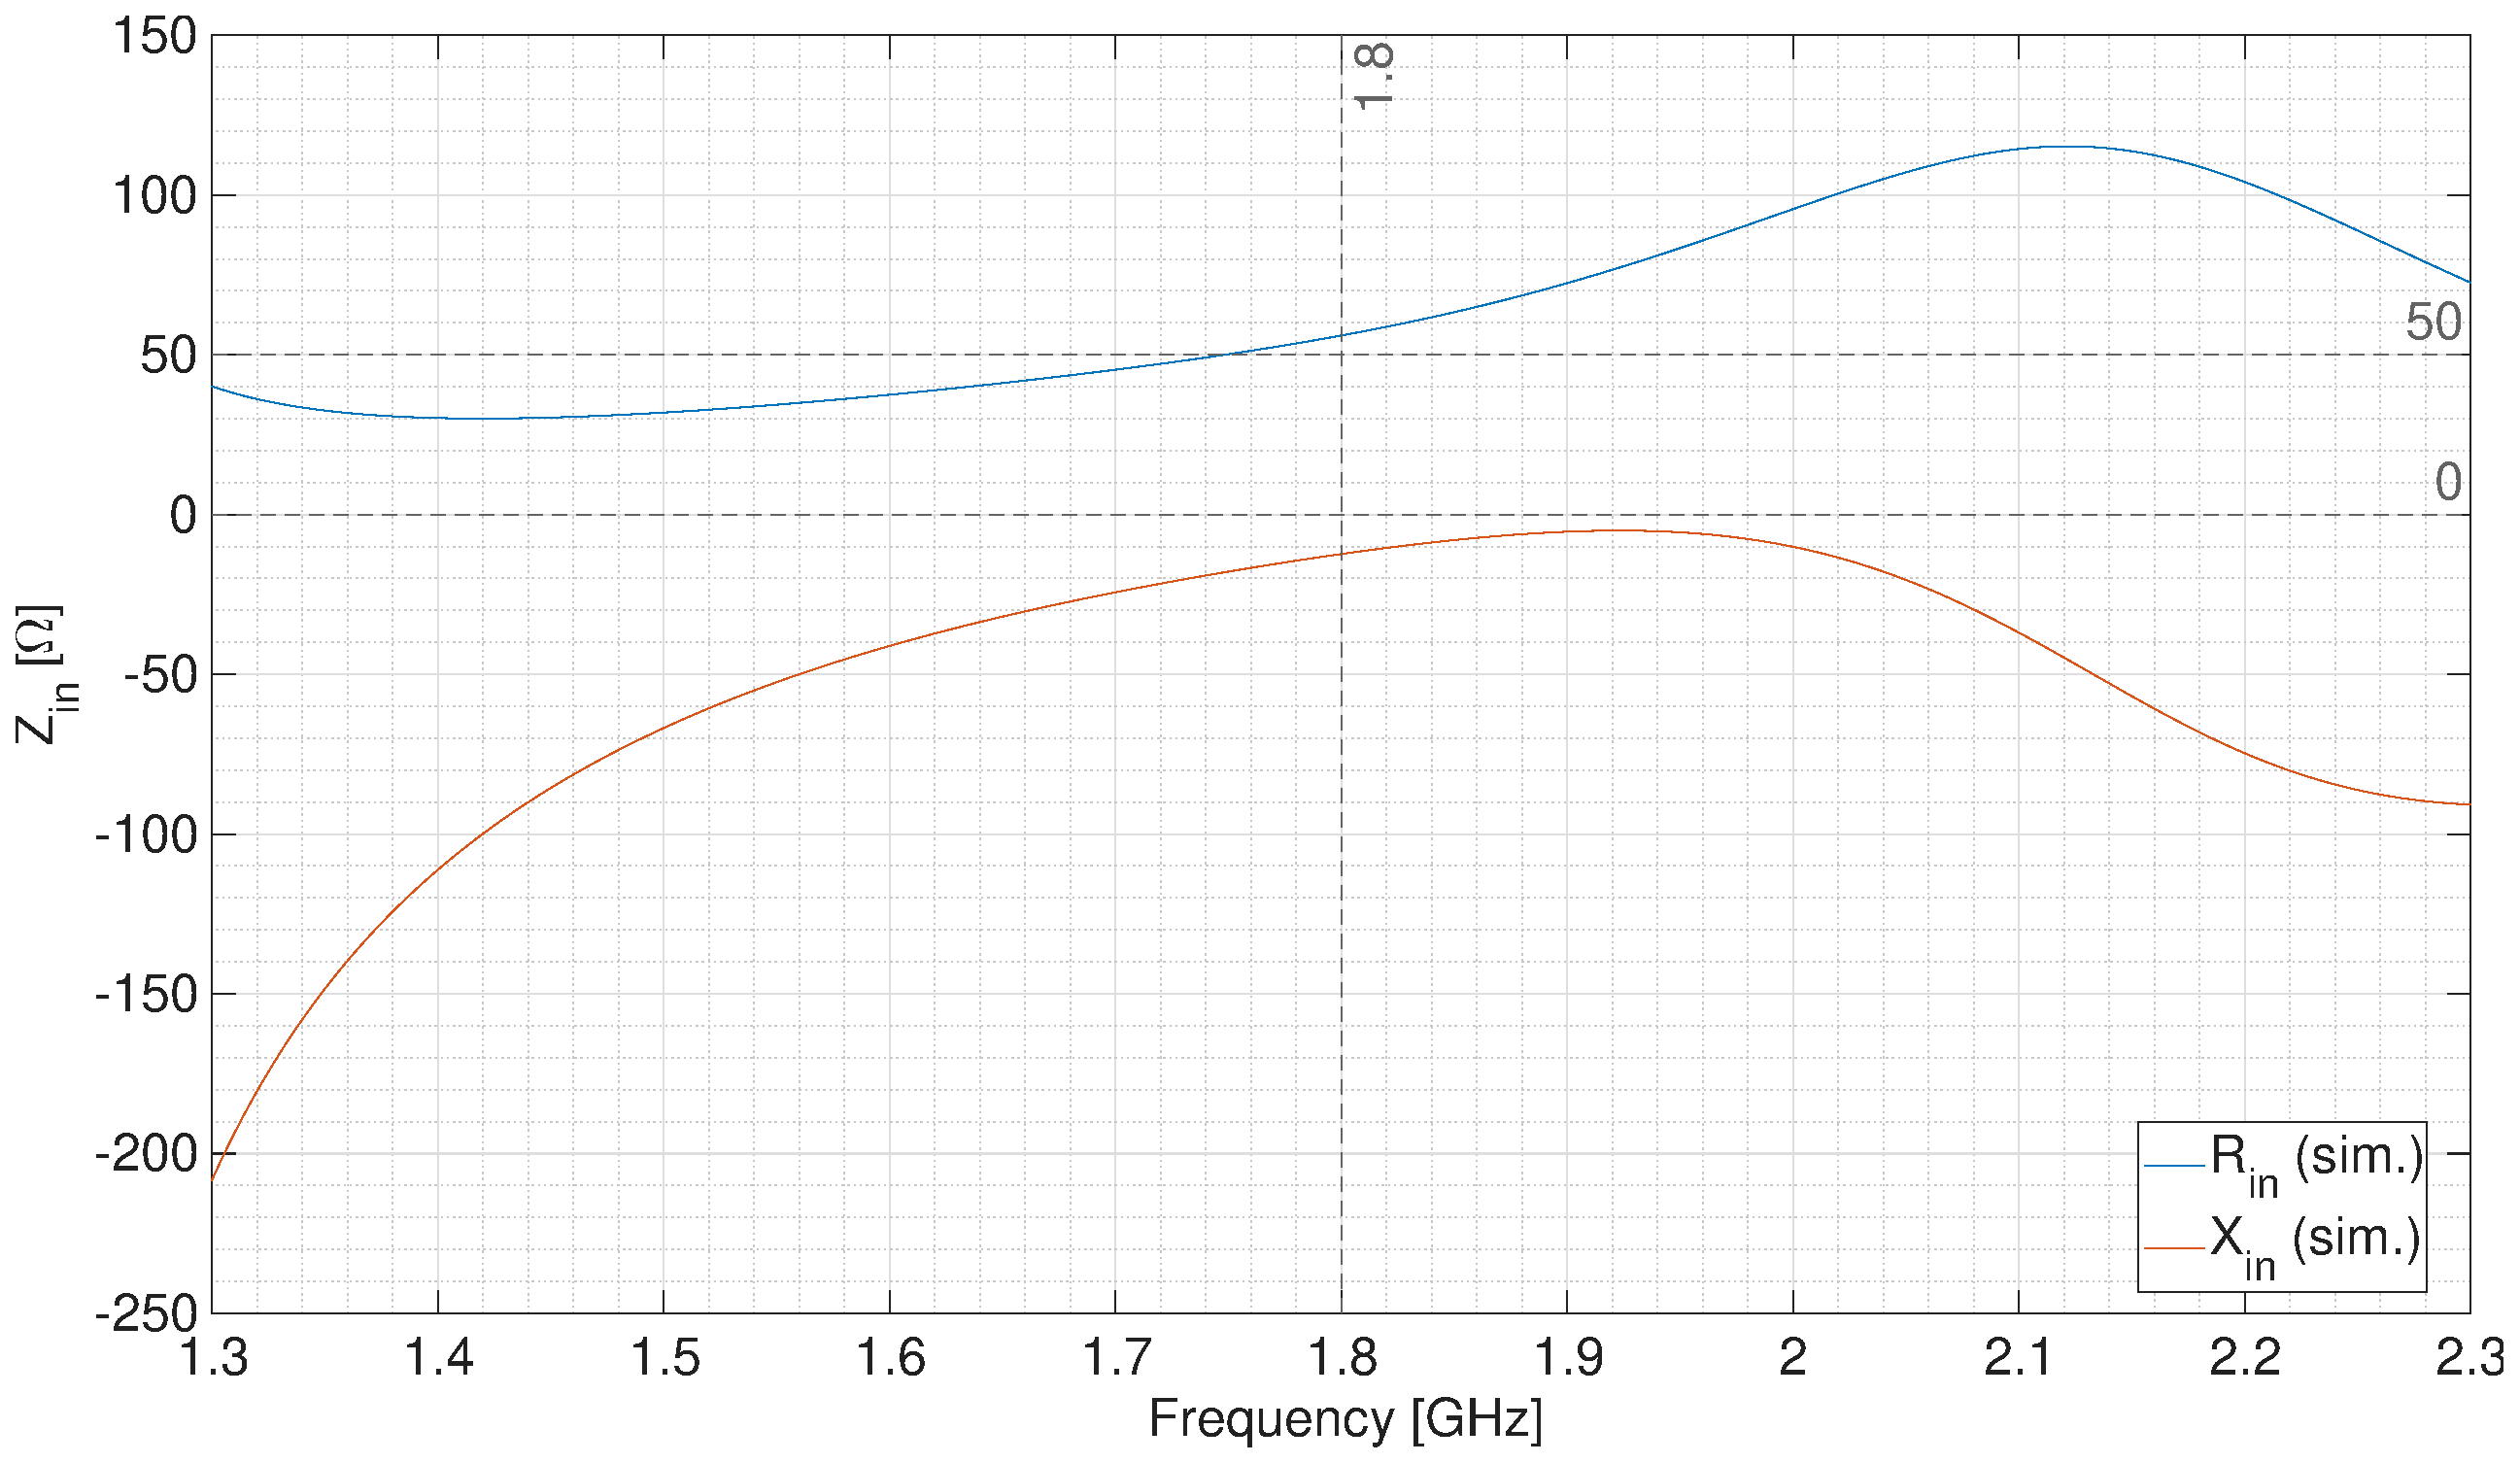
\includegraphics[width=.8\textwidth]{src/lambda-twentieth-impedance.eps}
            \caption{\label{fig:lambda-twentieth-impedance}Lambda-twentieth monopole: Input impedance}
        \end{figure}

\newpage
        \begin{figure}[!ht]
            \centering
            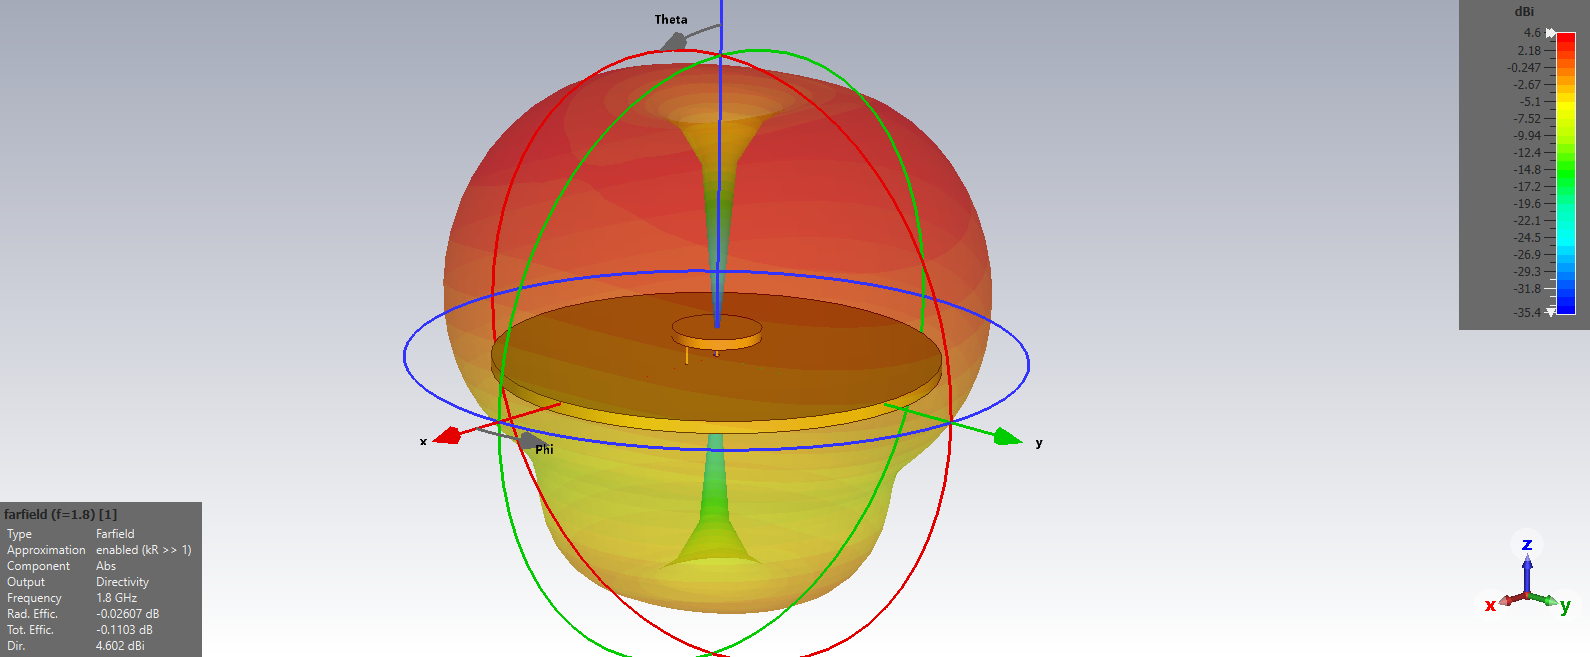
\includegraphics[width=.8\textwidth]{src/lambda-twentieth-farfield.png}
            \caption{\label{fig:lambda-twentieth-farfield}Lambda-twentieth monopole: farfield}
        \end{figure}

        \begin{figure}[!ht]
            \centering
            \begin{subfigure}{.4\textwidth}
                \centering
                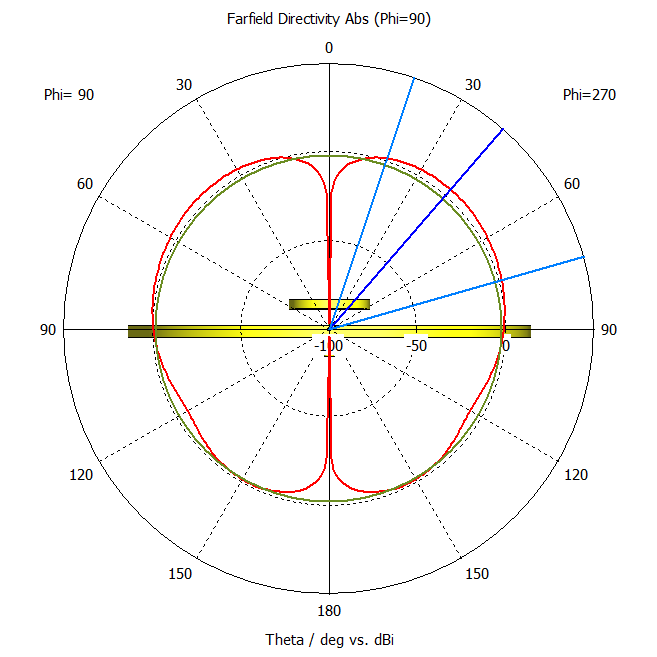
\includegraphics[width=\textwidth]{src/lambda-twentieth-radiation-e.png}
                \caption{\label{fig:lambda-twentieth-radiation-e}$E$-plane}
            \end{subfigure}
            ~
            \begin{subfigure}{.4\textwidth}
                \centering
                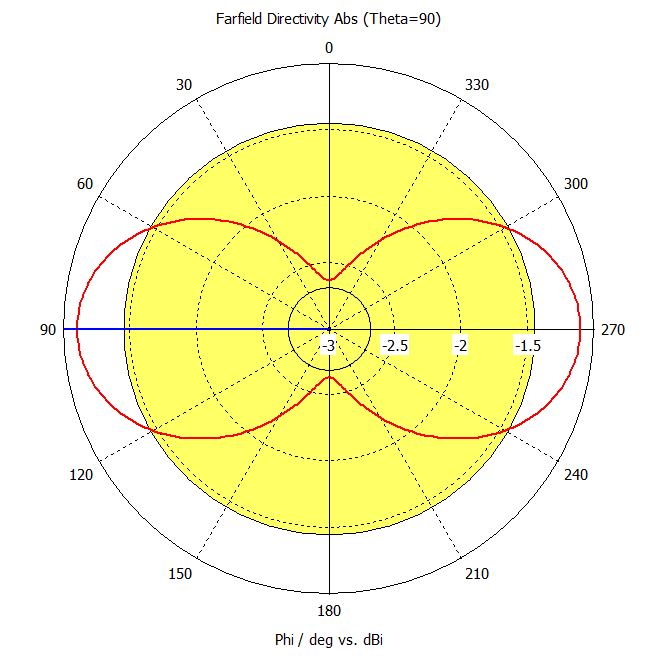
\includegraphics[width=\textwidth]{src/lambda-twentieth-radiation-h.png}
                \caption{\label{fig:lambda-twentieth-radiation-h}$H$-plane}
            \end{subfigure}
            \caption{\label{fig:lambda-twentieth-radiation}Lambda-twentieth monopole: radiation pattern cuts}
        \end{figure}

\newpage
        \section{Fundamental limits in the design bands}
            The Chu's fundamental limit of the quality factor with respect to the product $ka$ has been calculated according to the theoretical formulas
            \begin{align}
                Q_{\mathrm{McLean}} &= \frac{1}{(ka)^3} + \frac{1}{ka},
            &
                Q_{\mathrm{Thal}} &\approx \frac{1.5}{(ka)^3} + \frac{0.6}{ka},
            &
                Q_{\mathrm{Gustafsson}} &= \frac{1.5}{(ka)^3\gamma_1^{\mathrm{norm}}},
            \end{align}
            where $\gamma_1^{\mathrm{norm}}$ can be determined using available analytical formulas. Furthermore, quality factors of the designed antennas have been determined as $Q_{3\mathrm{dB}}$ from the 3 dB drop in reflection and $Q_Z$ from the input impedance using the formula
            \begin{align}
                Q_Z(\omega) &= \frac{\omega}{2R_{\mathrm{in}}(\omega)}\left|Z'_{\mathrm{in}}(\omega)\right|.
            \end{align}
            The resulting quality factors and their theoretical limits are shown in Figure~\ref{fig:quality-factor-limits} for both ways of determination.
            \begin{figure}[!ht]
                \centering
                \begin{subfigure}{.75\textwidth}
                    \centering
                    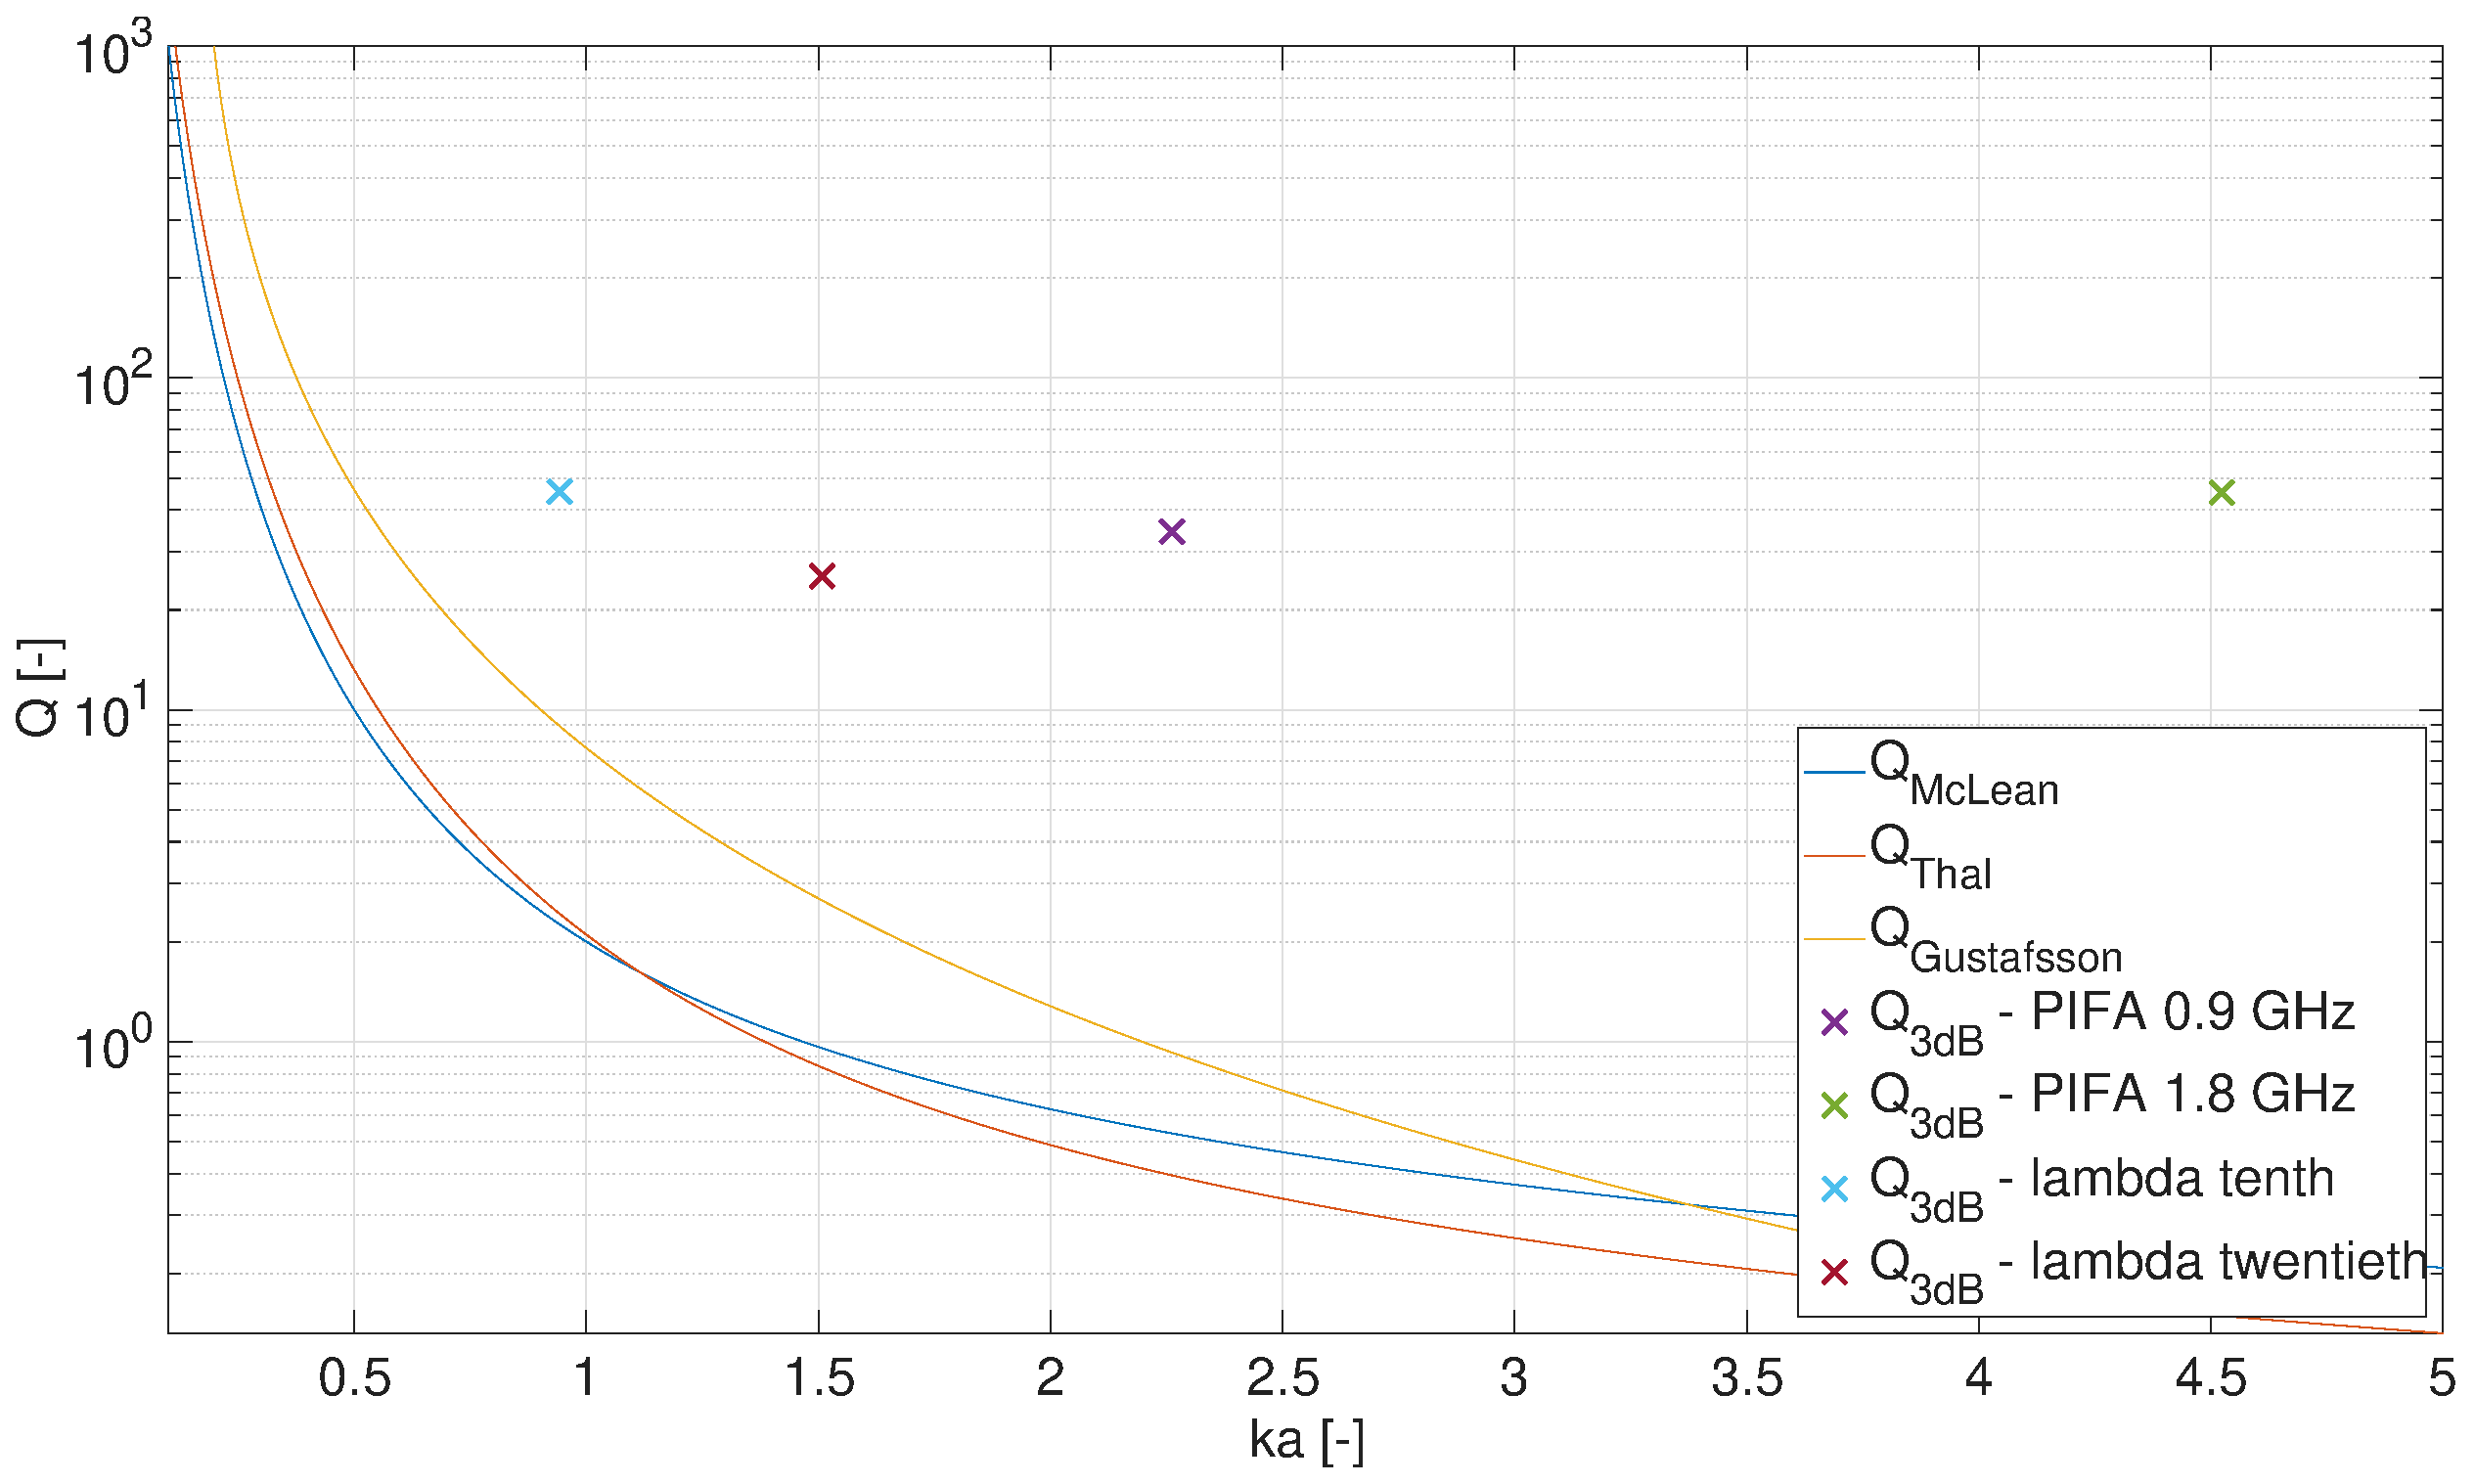
\includegraphics[width=\textwidth]{src/quality-factor-limits-q3db.eps}
                    \caption{\label{fig:quality-factor-limits-q3db}Quality factors calculated from the 3 dB drop in reflection}
                \end{subfigure}
                \\
                \centering
                \begin{subfigure}{.75\textwidth}
                    \centering
                    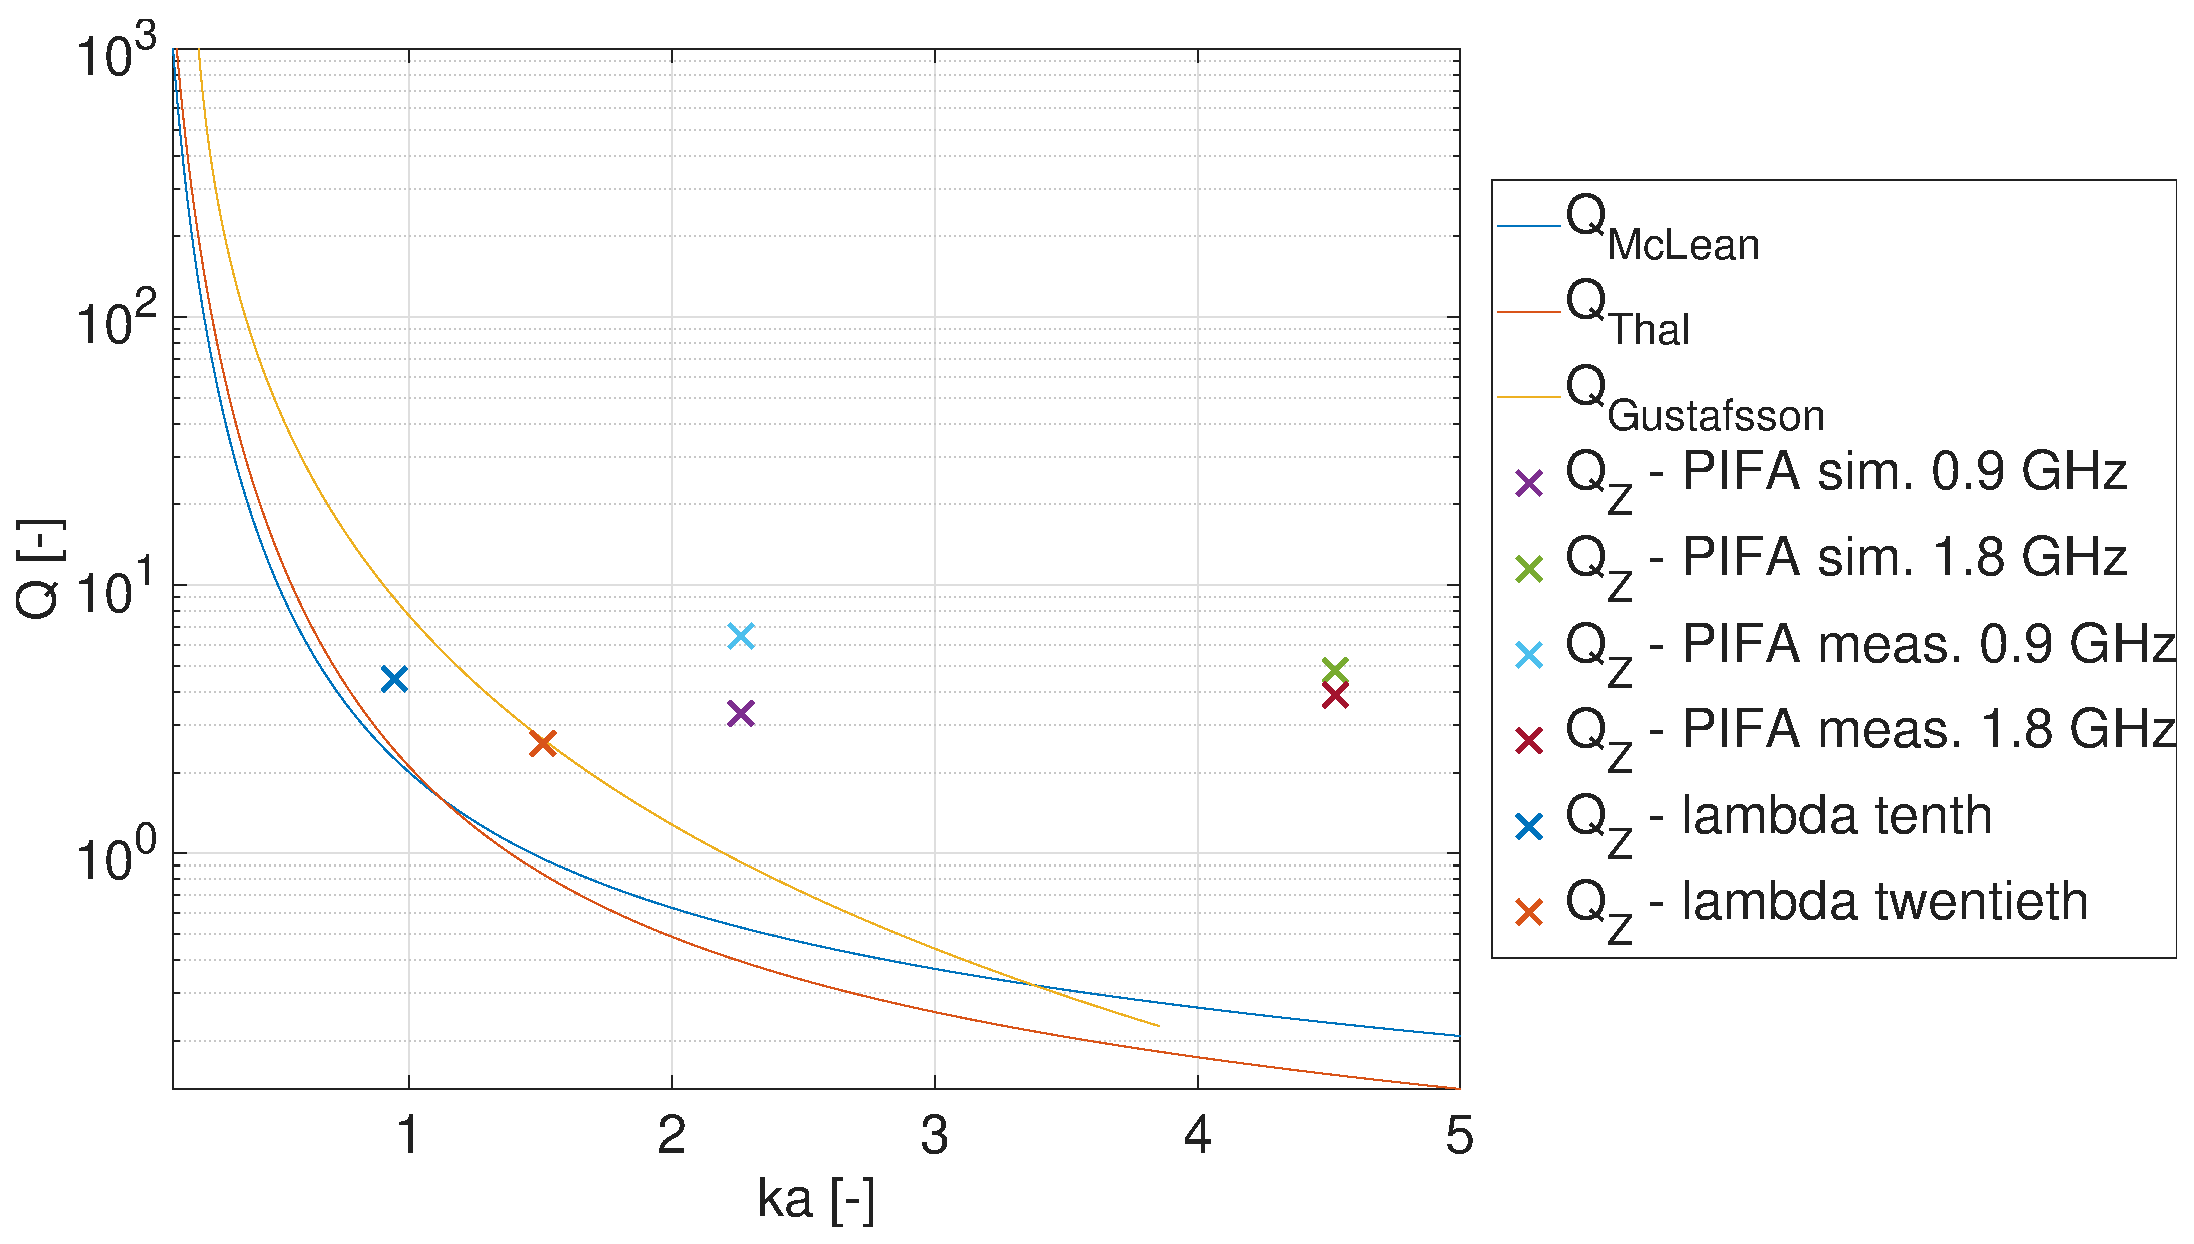
\includegraphics[width=\textwidth]{src/quality-factor-limits-qz.eps}
                    \caption{\label{fig:quality-factor-limits-qz}Quality factors calculated from input impedance}
                \end{subfigure}
                \caption{\label{fig:quality-factor-limits}Quality factors and their fundamental limits}
            \end{figure}

\newpage
            \paragraph{Discussion} The final resonance parameters including the quality factors (and their normalization to the Gustafsson's limit) and the resultant bandwidths are shown in Table~\ref{table:quality-factor-q3db} for the calculation from the 3 dB drop in reflection and in Table~\ref{table:quality-factor-qz} for the calculation from input impedance.
            \begin{table}[!ht]
                \centering
                \begin{tabular}{|c||c|c|c|c|}
                    \hline
                    Source & $ka\, [-]$ & $Q_{3\mathrm{dB}}\, [-]$ & $Q_{3\mathrm{dB}}/Q_{\mathrm{min}}\, [-]$ & $\mathit{BW}_{3\mathrm{dB}}\,[\%]$\\
                    \hline\hline
                    \makecell{PIFA (sim.)\\$0.9\, \mathrm{GHz}$} & $2.26$ & $34.47$ & $37.43$ & $5.82$\\
                    \hline
                    \makecell{PIFA (sim.)\\$1.8\, \mathrm{GHz}$} & $4.52$ & $45.16$ & $199.45$ & $4.44$\\
                    \hline
                    \makecell{$\lambda/10$\\monopole} & $0.94$ & $45.46$ & $5.16$ & $4.41$\\
                    \hline
                    \makecell{$\lambda/20$\\monopole} & $1.51$ & $25.31$ & $9.5$ & $7.92$\\
                    \hline
                \end{tabular}
                \caption{\label{table:quality-factor-q3db}Resonance parameters calculated from 3 dB drop in reflection}
            \end{table}

            \begin{table}[!ht]
                \centering
                \begin{tabular}{|c||c|c|c|c|}
                    \hline
                    Source & $ka\, [-]$ & $Q_Z\, [-]$ & $Q_Z/Q_{\mathrm{min}}\, [-]$ & $\mathit{BW}_Z\, [\%]$\\
                    \hline\hline
                    \makecell{PIFA (sim.)\\$0.9\, \mathrm{GHz}$} & $2.26$ & $3.32$ & $3.61$ & $20$\\
                    \hline
                    \makecell{PIFA (sim.)\\$1.8\, \mathrm{GHz}$} & $4.52$ & $4.81$ & $21.24$ & $14$\\
                    \hline
                    \makecell{PIFA (meas.)\\$0.9\, \mathrm{GHz}$} & $2.26$ & $8.78$ & $9.53$ & $8$\\
                    \hline
                    \makecell{PIFA (meas.)\\$1.8\, \mathrm{GHz}$} & $4.52$ & $11.31$ & $49.97$ & $6$\\
                    \hline
                    \makecell{$\lambda/10$\\monopole} & $0.94$ &  $4.46$ & $0.51$ & $15$\\
                    \hline
                    \makecell{$\lambda/20$\\monopole} & $1.51$ & $2.57$ & $0.96$ & $26$\\
                    \hline
                \end{tabular}
                \caption{\label{table:quality-factor-qz}Resonance parameters calculated from input impedance}
            \end{table}

            As we can see from the fundamental limits shown in Figure~\ref{fig:quality-factor-limits}, the quality factor is inversely proportional to the product $ka$. This implies that smaller antennas attain higher quality factor. This, however, brings issues in terms of low radiation efficiency and narrow bandwidth.
        

\end{document}
